% Options for packages loaded elsewhere
\PassOptionsToPackage{unicode}{hyperref}
\PassOptionsToPackage{hyphens}{url}
%
\documentclass[
]{article}
\usepackage{lmodern}
\usepackage{amssymb,amsmath}
\usepackage{ifxetex,ifluatex}
\ifnum 0\ifxetex 1\fi\ifluatex 1\fi=0 % if pdftex
  \usepackage[T1]{fontenc}
  \usepackage[utf8]{inputenc}
  \usepackage{textcomp} % provide euro and other symbols
\else % if luatex or xetex
  \usepackage{unicode-math}
  \defaultfontfeatures{Scale=MatchLowercase}
  \defaultfontfeatures[\rmfamily]{Ligatures=TeX,Scale=1}
\fi
% Use upquote if available, for straight quotes in verbatim environments
\IfFileExists{upquote.sty}{\usepackage{upquote}}{}
\IfFileExists{microtype.sty}{% use microtype if available
  \usepackage[]{microtype}
  \UseMicrotypeSet[protrusion]{basicmath} % disable protrusion for tt fonts
}{}
\makeatletter
\@ifundefined{KOMAClassName}{% if non-KOMA class
  \IfFileExists{parskip.sty}{%
    \usepackage{parskip}
  }{% else
    \setlength{\parindent}{0pt}
    \setlength{\parskip}{6pt plus 2pt minus 1pt}}
}{% if KOMA class
  \KOMAoptions{parskip=half}}
\makeatother
\usepackage{xcolor}
\IfFileExists{xurl.sty}{\usepackage{xurl}}{} % add URL line breaks if available
\IfFileExists{bookmark.sty}{\usepackage{bookmark}}{\usepackage{hyperref}}
\hypersetup{
  hidelinks,
  pdfcreator={LaTeX via pandoc}}
\urlstyle{same} % disable monospaced font for URLs
\usepackage{longtable,booktabs}
% Correct order of tables after \paragraph or \subparagraph
\usepackage{etoolbox}
\makeatletter
\patchcmd\longtable{\par}{\if@noskipsec\mbox{}\fi\par}{}{}
\makeatother
% Allow footnotes in longtable head/foot
\IfFileExists{footnotehyper.sty}{\usepackage{footnotehyper}}{\usepackage{footnote}}
\makesavenoteenv{longtable}
\usepackage{graphicx,grffile}
\makeatletter
\def\maxwidth{\ifdim\Gin@nat@width>\linewidth\linewidth\else\Gin@nat@width\fi}
\def\maxheight{\ifdim\Gin@nat@height>\textheight\textheight\else\Gin@nat@height\fi}
\makeatother
% Scale images if necessary, so that they will not overflow the page
% margins by default, and it is still possible to overwrite the defaults
% using explicit options in \includegraphics[width, height, ...]{}
\setkeys{Gin}{width=\maxwidth,height=\maxheight,keepaspectratio}
% Set default figure placement to htbp
\makeatletter
\def\fps@figure{htbp}
\makeatother
\setlength{\emergencystretch}{3em} % prevent overfull lines
\providecommand{\tightlist}{%
  \setlength{\itemsep}{0pt}\setlength{\parskip}{0pt}}
\setcounter{secnumdepth}{-\maxdimen} % remove section numbering

\date{}

\begin{document}

\begin{titlepage}
    \begin{center}
        
        \vspace*{2.5cm}
        
        \huge
        Is occupational asbestos exposure an under-recognised cause of idiopathic pulmonary fibrosis?
        \vspace{1.5cm}
        
        \Large
        Carl Jonathan Reynolds
        
        \vspace{1.5cm}

        \normalsize
        A thesis presented for the degree of\\
        Doctor of Philosophy
        
        \vfill
        
        \normalsize
        Supervised by:\\
        Professor Paul Cullinan\\
        Dr Chris Barber \\
        Dr Sara De Matteis

        \vspace{0.8cm}

        \normalsize
        Imperial College London, UK\\
        January 2020

         Except where otherwise noted, content in this thesis is licensed under a Creative Commons Attribution 4.0 License (http://creativecommons.org/licenses/by/4.0), which permits unrestricted use, distribution, and reproduction in any medium, provided the original work is properly cited. Copyright 2020, Carl Reynolds.

    \end{center}
\end{titlepage}

\vspace*{\fill}

\noindent \textit{
I, Carl Jonathan Reynolds confirm that the work presented in this thesis is my own. Where information has been derived from other sources, I confirm that this has been indicated in the thesis.
} \vspace*{\fill}

\setcounter{page}{2}

\hypertarget{abstract}{%
\section*{Abstract}\label{abstract}}
\addcontentsline{toc}{section}{Abstract}

The question of whether occupational asbestos exposure is an
under-recognized cause of idiopathic pulmonary fibrosis arises because
it is clinically plausible, epidemiologically plausible, and consistent
with fibre studies and case-control data. This thesis examines the
question by means of a literature review and a novel hospital based
case-control study, the idiopathic pulmonary fibrosis job exposures
study (IPFJES).

\hypertarget{acknowledgements}{%
\section*{Acknowledgements}\label{acknowledgements}}
\addcontentsline{toc}{section}{Acknowledgements}

I am grateful to Zeinab, Ada, and Rosa for putting up with me.

I am grateful to Paul, Chris, and Sara for their supervision.

I am grateful to the participants, to Rupa, and to all of the principle
investigators and their teams for helping to make the study happen.

\newpage

\tableofcontents

\newpage

\hypertarget{section}{%
\section*{}\label{section}}
\addcontentsline{toc}{section}{}

\listoffigures

\pagenumbering{roman}
\setcounter{page}{3}

\newpage

\hypertarget{list-of-tables}{%
\section*{List of tables}\label{list-of-tables}}
\addcontentsline{toc}{section}{List of tables}

Table 5.1 This is an example table . . . \hfill{pp}\\
Table x.x Short title of the figure . . . \hfill{pp}

To be added by Carl

\hypertarget{abbreviations}{%
\section*{Abbreviations}\label{abbreviations}}
\addcontentsline{toc}{section}{Abbreviations}

\begin{itemize}
\tightlist
\item
  \textbf{IPF} Idiopathic pulmonary fibrosis.
\item
  \textbf{MUC5B} Mucin 5B gene.
\item
  \textbf{IPFJES} Idiopathic pulmonary fibrosis job exposures study.
\item
  \textbf{JEM} Job exposure matrix.
\item
  \textbf{mMRC dyspnoea score} Modified Medical Research Council
  dyspnoea score.
\item
  \textbf{PMR} Proportional mortality rate.
\item
  \textbf{ONS} Office for National Statistics.
\item
  \textbf{SOC} Standard occupational classification.
\item
  \textbf{NS-SEC} National Statistics Socio-economic Classification.
\item
  \textbf{SNP} Single-nucleotide polymorphism.
\item
  \textbf{PCR} Polymerase chain reaction.
\item
  \textbf{GWAS} Genome wide association study.
\end{itemize}

\newpage

\hypertarget{introduction-to-thesis}{%
\section{Introduction to thesis}\label{introduction-to-thesis}}

\hypertarget{occupational-asbestos-exposure-as-an-under-recognised-cause-of-idiopathic-pulmonary-fibrosis}{%
\subsection{Occupational asbestos exposure as an under-recognised cause
of idiopathic pulmonary
fibrosis}\label{occupational-asbestos-exposure-as-an-under-recognised-cause-of-idiopathic-pulmonary-fibrosis}}

Idiopathic pulmonary fibrosis (IPF) is a progressive, fibrotic lung
disease which in 2016 was the recorded cause of death for approximately
5000 people in England and Wales. Its incidence, currently around
7.5/100,000 person-years, has increased by 5\% per annum in the period
1979-2016.{[}@Navaratnam2011{]}{[}@Navaratnam2019{]} The pathophysiology
of IPF is complex, the outcome of host susceptibility factors,
epithelial injury, and a dysregulated repair process. Several gene
polymorphisms which result in a vulnerable alveolar epithelium have been
characterized; they include abnormalities in mucin genes (eg MUC5B),
surfactant protein genes, and telomerase genes (eg TERT and
TERC).{[}@Maher2012{]}{[}@Ley2013{]}{[}@Spagnolo2014{]} The median age
of onset is 70 years and the condition is more common in men (M:F ratio
1.6), manual workers, and those living in industrial
areas{[}@Navaratnam2011{]}, patterns that are not unique to the
UK.{[}@Ley2013{]}{[}@Hutchinson2014{]} The prognosis is poor, with a
median survival of three years.{[}@Hubbard1998{]}{[}@Vancheri2010{]}

These epidemiological distributions of IPF are consistent with a
long-latency response to occupational dust exposure; in particular, the
incidence of IPF correlates strongly (if ecologically) with historic
asbestos use.{[}@Barber2015{]} Clinical, radiological, and
histopathological findings in asbestosis and IPF are
similar{[}@Corrin1985{]}{[}@Copley2003{]}. Mineralogical studies support
the concept of asbestosis-IPF misclassification by revealing high fibre
burdens in the lung tissue of patients diagnosed with `IPF' and revision
of the diagnosis to
`asbestosis'.{[}@Monso1990{]}{[}@Monso1991{]}{[}@Glazer2009{]}{[}@Ghio2014{]}

Establishing if occupational asbestos fibre exposure is an
under-recognised cause of IPF is an important step towards understanding
of the aetio-pathophysiology of IPF and the accuracy of prognostic
information. It would have implications for compensation and might
impact on the current restrictions on individual treatment. Importantly,
it would provide an additional data source to inform evidence-based
workplace exposure policies in the UK and internationally, particularly
in the many countries with continuing high levels of asbestos use.

\hypertarget{aims-and-objectives}{%
\subsection{Aims and objectives}\label{aims-and-objectives}}

My overall aim is to characterize and measure asbestos exposure as an
occupational determinant of IPF; additionally, I will determine
host-exposure interactions mediated by candidate susceptibility
polymorphisms (in particular MUC5B promoter polymorphism rs35705950).

My specific research questions are:

\begin{enumerate}
\def\labelenumi{\arabic{enumi}.}
\tightlist
\item
  Is there an association between occupational asbestos exposure and
  IPF?
\item
  Does a dose-response relationship exist for occupational asbestos
  exposure and IPF?
\item
  Does the presence of asbestos exposure modify the association between
  IPF and rs35705950?
\end{enumerate}

\hypertarget{data-sources}{%
\subsection{Data sources}\label{data-sources}}

\begin{itemize}
\tightlist
\item
  For the literature review and meta-analysis of occupational exposures
  in IPF I consider all published IPF case-control studies reporting on
  occupational exposures.
\item
  For the mortality analysis I use data obtained from the Office of
  National Statistics, Health and Safety Executive, and the World Health
  Organisation Mortality Database.
\item
  For brief reviews of asbestos exposure assessment and genetic
  susceptibility in IPF I rely on the published literature.
\item
  Primary case-control data collected during my PhD as part of the
  idiopathic pulmonary fibrosis job exposures study (IPFJES) is used to
  analyze asbestos exposure in IPF.
\end{itemize}

\hypertarget{outline-of-thesis}{%
\subsection{Outline of thesis}\label{outline-of-thesis}}

This chapter (Chapter 1) describes the problem studied, aims,
objectives, and approach. Chapter 2 is a literature review and
meta-analysis of IPF case-control studies that report on occupational
exposures. Chapter 3 is an analysis of IPF and asbestos related disease
mortality data. Chapter 4 is a review of asbestos exposure assessment
methodology. Chapter 5 is a review of the MUC5B promoter variant
rs35705950 in IPF. Chapter 6 describes the idiopathic pulmonary fibrosis
job exposures study (IPFJES) including results and analysis arising from
it. Chapter 7 concludes the thesis by summarising it and suggesting
future work.

\hypertarget{literature-review-and-meta-analysis-how-much-ipf-is-attributable-to-occupational-exposures}{%
\section{Literature review and meta-analysis: how much IPF is
attributable to occupational
exposures?}\label{literature-review-and-meta-analysis-how-much-ipf-is-attributable-to-occupational-exposures}}

\hypertarget{introduction}{%
\subsection{Introduction}\label{introduction}}

Idiopathic pulmonary fibrosis (IPF) is a diagnosis of exclusion. It is
made in the presence of a usual interstitial pneumonitis (UIP) pattern
on high resolution CT scan or biopsy. The diagnosis requires that known
causes of interstitial lung disease (such as drug toxicity, connective
tissue disease, domestic, and occupational or environmental exposures)
be excluded.{[}@Travis2013{]}

Attributing a disease process to a specific exposure can be difficult.
Disease processes are frequently complex or multifactorial, depending on
the interaction of genetic and environmental components. Well-studied
and relatively frequent entities such as chronic obstructive pulmonary
disease, ischaemic heart disease and diabetes lend themselves to
epidemiologic investigation, delineating the major risk factors for
disease and their relative contributions to risk at the population
level. IPF presents an additional challenge to attribution; because of
its relative infrequency, epidemiologic study of the disease is largely
limited to case-control studies.{[}@Reynolds2017{]} Studying specific
occupational exposures also presents its own challenges; co-exposure is
common, occupational hygiene data is frequently limited and
self-reported exposure is prone to recall bias.

I identified several review articles of the epidemiology of interstitial
lung disease that do not necessarily focus on IPF and only briefly
mention occupational factors (e.g Ley2013{[}@Ley2013{]}). Here I
consider review articles that specifically deal with occupational
factors in IPF and cite the case-control studies used.

Turner-Warwick (1998) discusses potential difficulties in establishing
attribution and causality in IPF. She observes that there is variation
in clinical practice with respect to the standard applied to exclude
IPF; some clinicians exclude IPF when exposure to a potential cause is
identified, others only when there is clear exposure to an established
cause. She explains that diagnosis based on radiologic and clinical
findings, and not on lung biopsy or bronchoalveolar lavage, may result
in initiating agents for disease being overlooked. Further, that
exposures such as asbestos, silica, coal, graphite, hard metal, and
avian proteins, may result in disease that can not be differentiated
from IPF.{[}@Turner-Warwick1998{]}

Reviewing the epidemiology of IPF and case-control studies to date
Hubbard (2001) describes the association of IPF with occupational
exposures to metal and wood and estimates that 10\% of IPF cases may be
due to occupational metal exposure and 5\% of cases to
wood.{[}@Hubbard2001{]}

Taskar and Coultas (2006) review and carry out a meta-analysis of six
case-control studies investigating environmental and occupational
exposures in IPF. They report population attributable risk percentages
for agriculture and farming (20.8\%), livestock (4.1\%), wood dust
(5\%), metal dust (3.4\%), stone/sand/silica (3.5\%), and smoking
(49.1\%).{[}@Taskar2006{]}

Gulati and Redlich's (2015) review of exposures causing UIP highlights
that asbestosis may appear indistinguishable from IPF and summarises
previous case-control studies but did not pool studies to perform a
meta-analysis.{[}@Gulati2015{]}

I sought to identify and meta-analyze all IPF case-control studies
dealing with occupational exposures. This work also contributed to a
joint ERS-ATS taskforce on the occupational burden of non-malignant
respiratory disease.{[}@Blanc2019{]}

\hypertarget{method}{%
\subsection{Method}\label{method}}

I searched Pubmed, embase, and google scholar databases for combinations
of the terms `idiopathic pulmonary fibrosis', `occupation',
`case-control study' and synonyms. My search included all publications
from published from the respective database start dates until September
2018. When I identified a relevant paper I also reviewed the references
and papers citing the paper. I also used Medline
ranker{[}@Fontaine2009{]} and bespoke pubmed `mining'
techniques.{[}@Reynolds2017pubmed{]}

A colleague independently reviewed and abstracted data for five exposure
categories common to the identified case-control studies: ``vapors,
gases, dusts, and/or fumes (VGDF)'', ``metal dust'', ``wood dust'',
``silica dust'', and ``agricultural dust''. I calculated PAF as follows:
PAF=pc(OR - 1)/OR, where pc is the proportion of cases exposed and OR is
the risk estimate.

I calculated pooled OR and pooled PAF for occupational exposures using
fixed effects models and random effects models in Stata (StataCorp.
2015. Stata Statistical Software: Release 14. College Station, TX:
StataCorp LP). When there was results of the models differed
substantively, we used the results of the fixed effects model, which
were more conservative. The pooled PAF relied on the ratio of
attributable cases to all cases underlying each risk estimate.

\hypertarget{results}{%
\subsection{Results}\label{results}}

I found (as of September 2018) 15 case-control studies looking at
occupational exposures in IPF; the most recent review
article{[}@Gulati2015{]} covers only eight of them. Associations with
metal, wood, silica, and agricultural dust were reported.
{[}@Scott1990{]} {[}@Iwai1994{]} {[}@Hubbard1996a{]} {[}@Mullen1998{]}
{[}@Baumgartner2000{]} {[}@Hubbard2000{]} {[}@Miyake2005{]}
{[}@Gustafson2007{]} {[}@Pinheiro2008{]}
{[}@Garcia-SanchoFigueroa2010{]} {[}@Garcia-Sancho2011{]}
{[}@Awadalla2012{]} {[}@Paolocci2013{]} {[}@Ekstrom2014{]}
{[}@Koo2017{]} One study{[}@Paolocci2013{]} was included even though it
was only available as an abstract at the time of analysis because we
knew the fulltext paper was forthcoming.{[}@Paolocci2018{]} All figures
are adapted from Blanc et al 2019.{[}@Blanc2019{]}

\begin{figure}
\centering
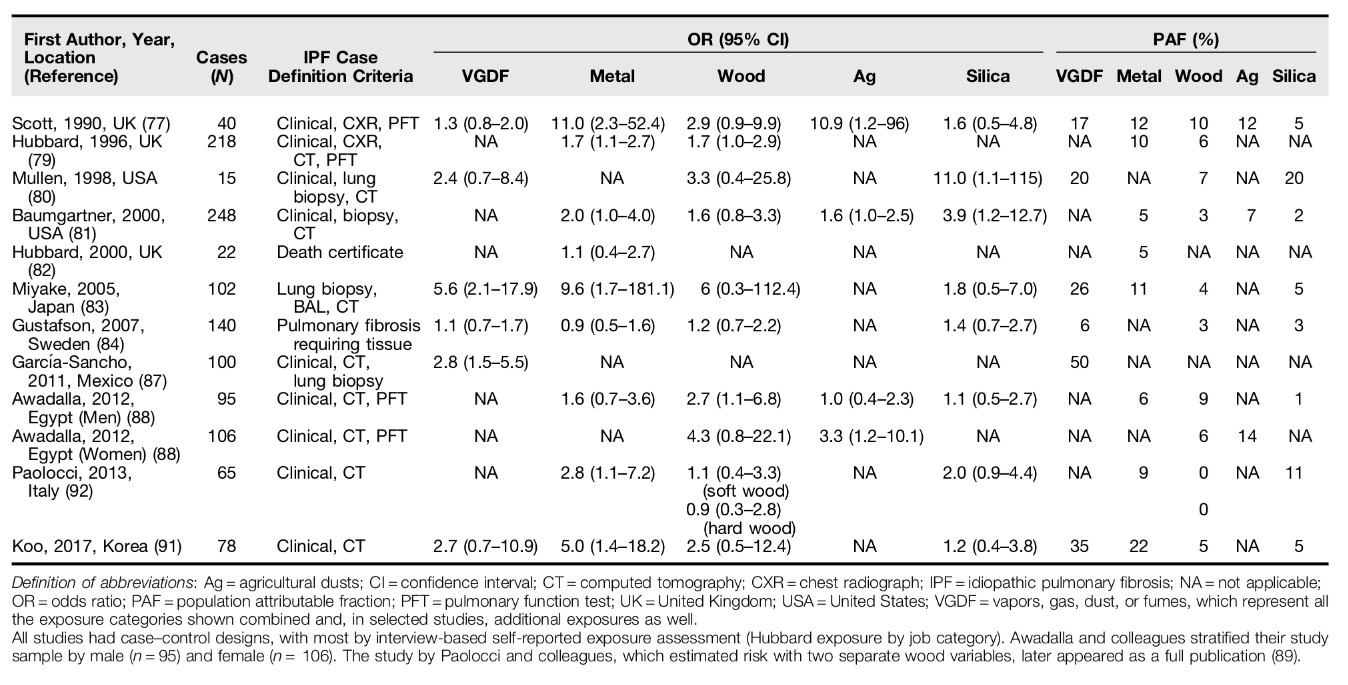
\includegraphics{source/figures/prevstudies.jpg}
\caption{Previous IPF case-control studies reporting on occupational
exposures. (Blanc 2019)}
\end{figure}

I used 40 risk estimates from 12 publications (1326 IPF cases in total)
to perform a metanalysis.{[}@Scott1990{]} {[}@Hubbard1996a{]}
{[}@Mullen1998{]} {[}@Baumgartner2000{]} {[}@Hubbard2000{]}
{[}@Miyake2005{]} {[}@Gustafson2007{]} {[}@Garcia-SanchoFigueroa2010{]}
{[}@Garcia-Sancho2011{]} {[}@Awadalla2012{]} {[}@Paolocci2013{]}
{[}@Koo2017{]} Three studies were not used, one because data was not
collected on the proportion of cases with specific occupational
exposures{[}@Iwai1994{]}, one because of methodological differences in
exposure assignment{[}@Pinheiro2008{]}, and one because if reported data
for pulmonary fibrosis rather than IPF.{[}@Ekstrom2014{]} Each exposure
category was assessed with 6-11 risk estimates (Table 2.2).

\begin{figure}
\centering
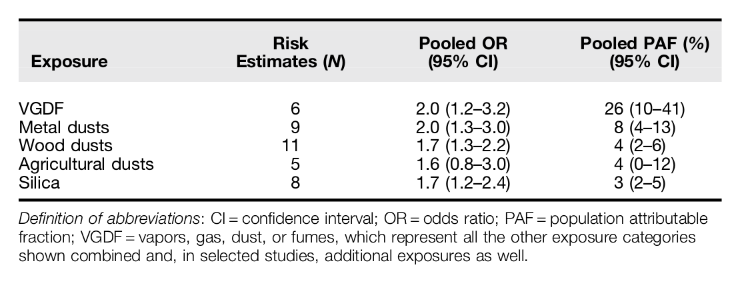
\includegraphics{source/figures/paf.png}
\caption{Pooled population attributable risk factors for occupation and
idiopathic pulmonary fibrosis. (Blanc 2019)}
\end{figure}

\begin{figure}
\centering
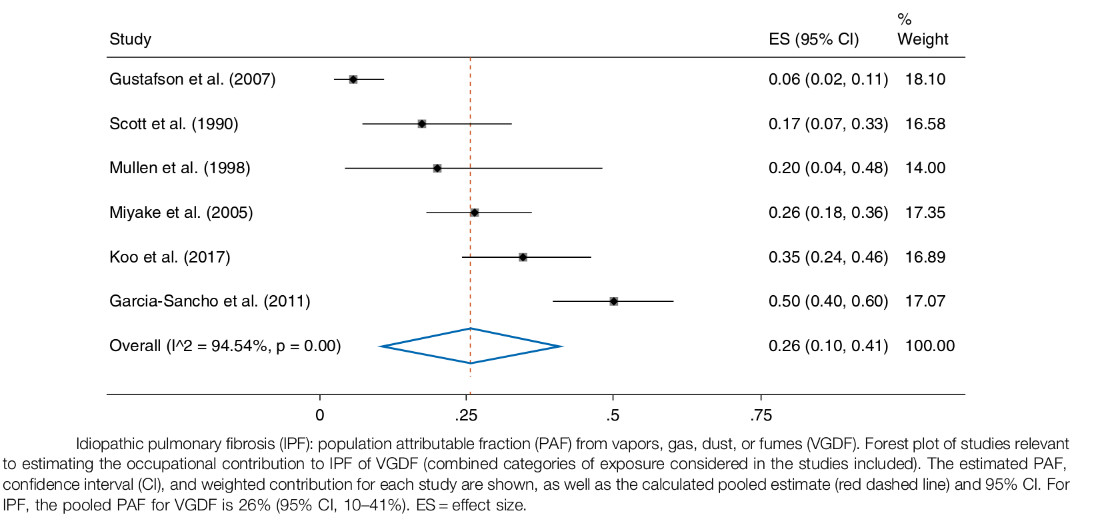
\includegraphics{source/figures/forrest.jpg}
\caption{Forrest plot of pooled population attributable risk factors for
occupational VGDF exposure and idiopathic pulmonary fibrosis. (Blanc
2019)}
\end{figure}

\hypertarget{discussion}{%
\subsection{Discussion}\label{discussion}}

My results support the case for a proportion of IPF cases being
attributable to occupational exposures.

Pooled ORs were significantly elevated for VGDF, metal dust, wood dust,
agricultural dust, and silica dust; the pooled PAF estimates by category
ranged from 4-23\%. This is an important finding for an otherwise
idiopathic disease which carries significant morbidity and mortality;
identifying causal occupational agents could permit remediation and
prevention.

Associations between IPF and wood, metal, and agricultural dust were
previously reported in a meta-analysis of six case-control studies by
Taskar and Coultas. {[}@Taskar2006{]} While my findings are similar I
found a smaller effect size for agricultural exposure and a large effect
size for non-specific vapours, gases, dust, and fumes (VGDF), see Table
2.2.

Funnel plot asymmetry using Egger's test, which may be due to
publication bias, was present for VGDF (p = 0.04) and metal dust (p =
0.03) but not for wood dust (p = 0.09), silica dust (p = 0.2), and
agricultural dust (p = 0.6). However, the number of studies included is
small and funnel plot assymetry may be due to chance rather than bias.

There are several limitations to the meta-analysis that arise from the
case-control studies included.

Several studies {[}@Scott1990{]} {[}@Hubbard1996{]}
{[}@Baumgartner2000{]} {[}@Gustafson2007{]} {[}@Garcia-Sancho2011{]}
used population controls but do not provide details on participation
rates. Participation rates can be low for community controls; a recent
UK case-control study investigating prothrombotic factors in IPF
reported a response rate of 28\% for commumnity controls.
{[}@Navaratnam2014{]} This approach is vulnerable to non-responder bias.
One study{[}@Hubbard2000{]} used employee occupational records and death
certificates from pension-fund records for a single company and was only
able to locate the occupational records for 40\% of cases and 38\% of
controls.

Nearly all studies relied on self-reported exposures rather than life
time occupational histories to assess exposure; an approach that is
prone to recall bias and does not permit examination of dose-response
relationships.

Reliance on self-reported exposures also means that studies are
potentially vulnerable to confounding as a result of co-exposure. For
example, several studies have described strong associations between
metal work and IPF and specify sheet metal
workers{[}@Iwai1994{]}{[}@Scott1990{]}{[}@Hubbard2000{]}, a group who
are frequently exposed to dust containing asbestos
fibres{[}@Welch1994{]} and who in a recent UK study, had the highest
risk of mesothelioma.{[}@Rake2009{]}

Case definitions and sources for cases varied between studies. For
example Scott (1990){[}@Scott1990{]} used a case definition which
included a chest radiograph showing bilateral interstitial shadowing
whereas most other studies relied on high resolution CT. Four studies
used mortality data
{[}@Iwai1994{]}{[}@Pinheiro2008{]}{[}@Gustafson2007{]}{[}@Hubbard2000{]}
to identify cases and one study{[}@Gustafson2007{]} used a national
register of patients receiving oxygen therapy. Differences in healthcare
coverage and coding practices can result in selection
bias.{[}@Caminati2015{]}

\hypertarget{conclusion}{%
\subsection{Conclusion}\label{conclusion}}

The observed excess risk could represent disease misclassification of
pneumoconiosis or hypersensitivity pneumonitis, but this is unlikely to
fully explain the observed effects. My analysis supports an etiologic
role for occupational exposures in IPF, potentially explaining up to
23\% of the burden of disease and highlighting a role for workplace
exposure reduction in disease prevention.

\hypertarget{mortality-analysis-do-mortality-trends-support-an-occupational-cause}{%
\section{Mortality analysis: do mortality trends support an occupational
cause?}\label{mortality-analysis-do-mortality-trends-support-an-occupational-cause}}

\hypertarget{introduction-1}{%
\subsection{Introduction}\label{introduction-1}}

The incidence of Idiopathic pulmonary fibrosis (IPF) has been increasing
at an average rate of 5\% per annum for the period 1979 to
2016.{[}@Navaratnam2019{]} By definition, the diagnosis of IPF is not
made in the presence of an identifiable cause. However, the distribution
of the disease in the population (more common in men, manual workers,
and those living in more industrial areas of the country) suggests a
causal contribution from an occupational or environmental source.

I hypothesised that a proportion of Idiopathic Pulmonary Fibrosis (IPF)
cases are due to occult environmental or occupational exposures to
asbestos dust. This would be expected to result in a spatio-temporal
association between IPF, Mesothelioma, and Asbestosis mortality patterns
coinciding with asbestos exposure. It would also be expected to produce
a birth cohort effect.

I examined trends in IPF, Mesothelioma, and Asbestosis mortality data
for evidence of cohort effect and association.

\hypertarget{method-1}{%
\subsection{Method}\label{method-1}}

I obtained regional age and sex stratified mortality data for IPF,
Mesothelioma, and Asbestosis for England and Wales from the Office of
National Statistics for the period 1974--2012. Data were
age-standardised and visualised using the Python Pandas data analysis
library and matplotlib. For regional analysis poisson regression of
counts was used adjusting for age and sex.

\hypertarget{results-1}{%
\subsection{Results}\label{results-1}}

IPF, mesothelioma, and asbestosis mortality rates increased thorough the
study period. IPF increased at a rate of approximately 5\% per annum.
The Female:Male for IPF is approximately 1:1.6 and there are more IPF
deaths in the North West and South East of England. IPF mortality does
appear to correlate with mesothelioma mortality (Figure
\ref{mortalitytrends}). There is evidence of a cohort effect with
age-specific IPF death rates increasing in successive cohorts, most
clearly seen from age 60 (Figure \ref{birthcohorts}). While overall
rates were higher for men but there were not marked sex differences in
cohort mortality trends. There was not a clear relationship in regional
mortality for IPF, Mesothelioma, and Asbestosis (Table 1).

\begin{figure}
\centering
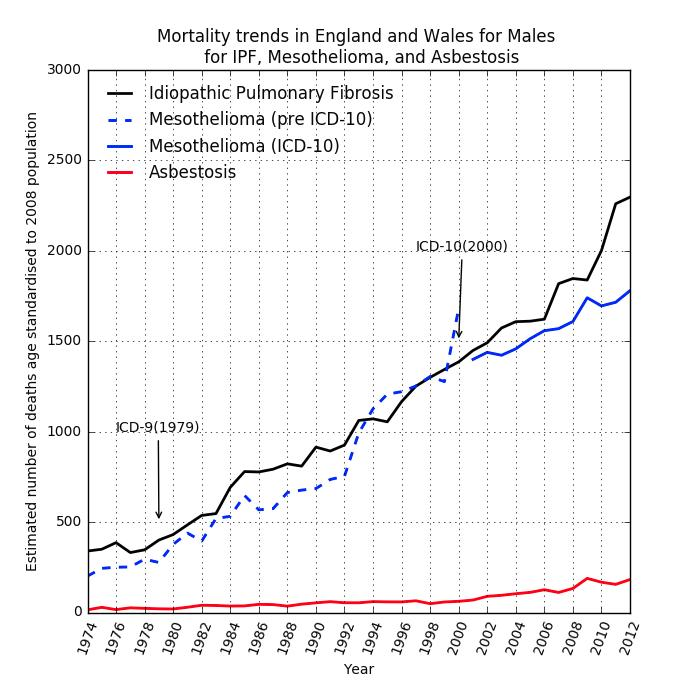
\includegraphics[width=0.5\textwidth,height=\textheight]{source/figures/ipfasbmesomaletrend.jpg}
\caption{IPF, mesothelioma, and asbestosis mortality trends
\label{mortalitytrends}}
\end{figure}

\begin{figure}
\centering
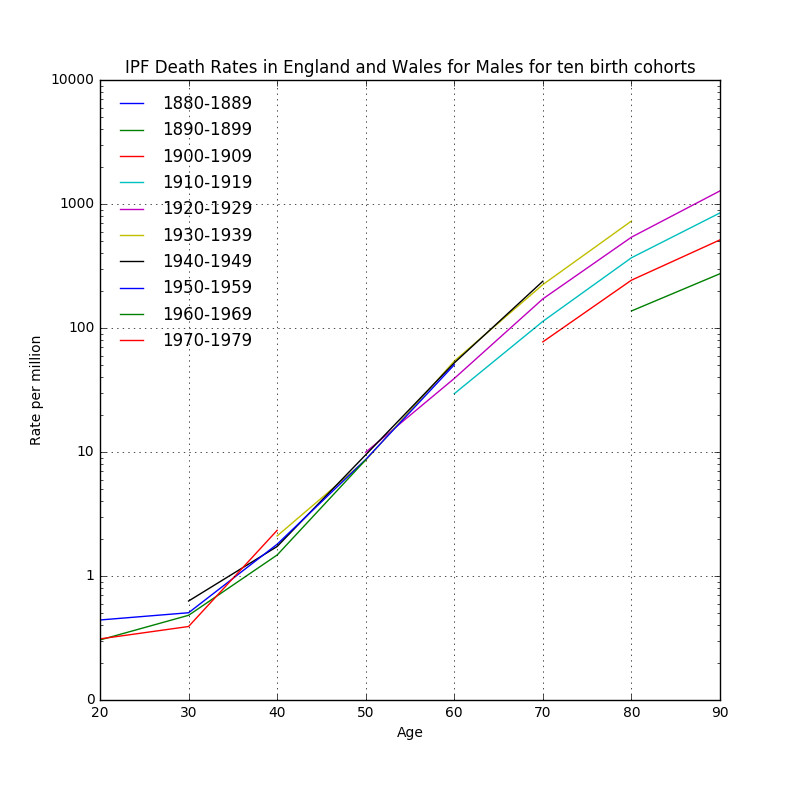
\includegraphics[width=0.5\textwidth,height=\textheight]{source/figures/ipfmalebirthcohorts.jpg}
\caption{IPF male birth cohort age-specific mortality rates per million
1880-1979 \label{birthcohorts}}
\end{figure}

\hypertarget{table-1-regional-ipf-mesothelioma-and-asbestosis-mortality-1974-2012.-or-95ci.}{%
\subsubsection{Table 1: Regional IPF, Mesothelioma, and Asbestosis
mortality 1974-2012. OR
(95\%CI).}\label{table-1-regional-ipf-mesothelioma-and-asbestosis-mortality-1974-2012.-or-95ci.}}

\begin{longtable}[]{@{}llll@{}}
\toprule
Region & IPF & Mesothelioma & Asbestosis\tabularnewline
\midrule
\endhead
North West & 1.3(1.26-1.35) & 0.99(0.95-1.03) &
2.28(1.89-2.74)\tabularnewline
Wales & 1.28(1.23-1.33) & 0.61(0.58-0.65) &
1.09(0.84-1.4)\tabularnewline
North East & 1.24(1.19-1.29) & 1.71(1.64-1.79) &
5.7(4.74-6.86)\tabularnewline
West Midlands & 1.2(1.16-1.24) & 0.76(0.73-0.8) & 1.19
(0.95-1.48)\tabularnewline
East Midlands & 1.16(1.12-1.21) & 0.78(0.75-0.82) & 1.4
(1.12-1.74)\tabularnewline
Yorkshire and the Humber & 1.11(1.07-1.15) & 1.1(1.06-1.15) &
1.62(1.32-1.98)\tabularnewline
South West & 1.1(1.06-1.13) & 0.87(0.83-0.9) &
1.81(1.49-2.2)\tabularnewline
London & 1.01(0.97-1.05) & 1(0.96-1.04) & 2.15(1.77-2.6)\tabularnewline
South East & 0.9(0.87-0.93) & 0.95(0.92-1.31) &
1.31(1.09-1.59)\tabularnewline
East & 1 & 1 & 1\tabularnewline
\bottomrule
\end{longtable}

\hypertarget{discussion-1}{%
\subsection{Discussion}\label{discussion-1}}

I found evidence of a cohort effect whereby age specific-specific IPF
death rates have increased in successive cohorts. These findings are
similar to a recent study by Navaratnam et al using the same data
source{[}@Navaratnam2019{]} and mesothelioma birth cohort age adjusted
mortality trends.{[}@Darnton2012{]}

Mortality data for IPF has the advantage of capturing a sufficiently
large number of deaths to permit analysis of trends over time with a
reasonable degreee of confidence. The accuracy of reports over time may
have varied, this is a potential consequence of coding changes since
prior to 2000, and the use of ICD-10, there was not a unique code for
IPF and thus some ambiguity as to how it should be coded. However, a
death certification validation study using an IPF cohort of 211 incident
cases diagnosed in England and Wales between 2010 to 2012 found that of
the 124 deaths occuring in study period 83(67\%) had IPF coded as the
underlying cause of death and 102(82\%) had it coded anywhere on the
death certificate.{[}@Hutchinson2014{]} Therefore capture is good and
estimates of disease prevelence based on mortality are likely to be
conservative.

The close correlation between IPF and mesothelioma mortality in the UK
has been observed by others{[}@Barber2015{]} who reported pearson
correlation coefficients of 0.98 (p\textless0.001) for men and
0.97(p\textless0.001) for women and noted that lagged historic asbestos
imports also correlate strongly with IPF and mesothelioma mortality in
the UK. Alternative explanations for the rise in IPF cases include
increased recognition of cases{[}@Navaratnam2019{]} and overdiagnosis on
the basis of CT criteria.{[}@Wells2013{]}

\hypertarget{conclusion-1}{%
\subsection{Conclusion}\label{conclusion-1}}

There is an unexplained sustained increase in the incidence of IPF and a
very suggestive, if ecological, association with mesothelioma and lagged
historic asbestos imports. There does appear to be a birth cohort effect
whereby age specific rates are higher in later cohorts that would, for
the data considered, be consistent with historic occupational asbestos
exposure and a long latency between exposure and disease.

\hypertarget{historic-asbestos-exposure-assessment-can-it-be-done}{%
\section{Historic asbestos exposure assessment: can it be
done?}\label{historic-asbestos-exposure-assessment-can-it-be-done}}

\hypertarget{introduction-2}{%
\subsection{Introduction}\label{introduction-2}}

Asbestos related respiratory disease is initiated by inhalation of
asbestos fibres. In the UK clinically significant asbestos exposure is
largely occupational and, as a result of asbestos control legislation,
historic.

Occupational asbestos exposure can be assessed quantitatively by
sampling ambient air at a workplace and calculating a fibre count using
microscopy. Alternatively, because inhaled asbestos fibres persist in
the lung they can be sampled by lung biopsy, bronchoalveolar lavage, or
at autopsy.

Historic workplace measurements are a valuable resource for assessing
exposure but are limited in several ways. Measurements are not available
for many occupations, where measurements are available they are
dependant on working practices and measurement technique at the time of
assessment; they do not necessarily generalize well.

Measurement of asbestos fibres in lung tissue by means of biopsy or
bronchoalveolar lavage is invasive and both procedures carry the risk of
serious complication including death. Additionally, the biopersistence
of asbestos fibres is variable, the physical characteristics of inhaled
fibres may be modified in-situ{[}@Mossman2011{]}, counts are sensitive
to techniques used, and establishing appropriate references ranges is
challenging.{[}@DeVuyst1998{]}

Expert assessment and exposure modelling approaches integrate historic
workplace measurements with simulated workplace measurements and an
individuals recollection of job processes he or she has carried out
during their working life.{[}@Cherrie1999{]}

Job-exposure matrices (JEMs) are widely used in occupational
epidemiology studies to assess exposure to potential hazards. These
assign levels of exposure to health hazards on the basis of job title.

Finally, self-reported exposures are a subjects direct report of what
they have been exposed to, these are usually elicited by questionnaire
or at interview.

The asbestos exposure assessment literature presents difficulties for
review because it is large and recognised to be at risk of bias as a
result of its economic importance to powerful industrial and medicolegal
actors{[}@Nemery2017{]}.

Here I critically review different means of historic asbestos exposure
assessment and consider their clinical and research utility.

\hypertarget{method-2}{%
\subsection{Method}\label{method-2}}

I searched pubmed and google scholar for combinations and synonyms of
``asbestos'', ``exposure assessment'', together with terms for modes of
assessment including ``lung biopsy'', ``bronchoalveolar lavage'',
``exposure reconstruction'', and ``job-exposure matrix''. When a
relevant papers was identified, papers referenced, and papers citing,
the paper were reviewed.

\hypertarget{results-2}{%
\subsection{Results}\label{results-2}}

\hypertarget{lung-biopsy-and-bronchoalveolar-lavage}{%
\subsubsection{Lung biopsy and bronchoalveolar
lavage}\label{lung-biopsy-and-bronchoalveolar-lavage}}

The first report of fibrosis of the lung due to asbestos
dust{[}@Cooke1924{]} included a description of the post mortem
microscopic appearances of the lungs which showed abundant asbestos
fibres in areas of fibrosis.

The demonstration of asbestos fibres on lung biopsy in the context of
pulmonary fibrosis is clearly supportive of the diagnosis of asbestosis.
However, a failure to demonstrate fibres can not be used to rule out
asbestos exposure because fibres, particularly chrysotile fibres, may be
cleared from the lung and counting methods have a significant
false-negative rate.{[}@DeVuyst1998{]}

Despite this recent 2014 Helsinki guidelines{[}@Wolff2015{]} and UK
Royal College of Pathologists guidelines appear to suggest that a clear
history of substantial occupational asbestos exposure is insufficient
for diagnosis and that the absence of asbestos bodies or fibre counts
above a certain threshold may be used to rule out the diagnosis. The
shortcomings of such an approach highlighted above are also described by
responses to the Helsinki
guideline.{[}@Hammar2015{]}{[}@Baur2016{]}{[}@Baur2017{]}

Lung biopsy carries significant health risks, particularly for patients
who already have compromised lung function and it can not be justified
solely on medico-legal grounds.{[}@Baur2016{]} Therefore, the clinical
utility of lung biopsy and bronchoalveolar lavage is limited to ruling
in asbestosis when a suggestive exposure history and radiology are
lacking.

In a research context lung biopsy and bronchoalveolar lavage have
provided valuable population level insights. Lung biopsy asbestos fibre
counts have been examined in a UK case-control study where mesothelioma
cases were compared with lung cancer controls. Fibre counts were found
to be higher in groups with greater occupational risk (as defined by
PMR), providing additional support for the pre-eminence of an
occupational history.{[}@Rake2009{]}{[}@Gilham2016{]} In a follow up
study asbestos fibre counts from unselected surgically treated
pneumothorax patients were used to demonstrated that population
amphibole burden is falling and is proportional to mesothelioma
mortality.{[}@Gilham2018{]}

A similar correlation with occupational exposure history, overall
downward trend in fibre counts, and a significant false negative rate
has been observed in a recent Belgian study of patients undergoing
bronchoscopy with bronchoalvelolar lavage sampling for asbestos fibre
quantification.{[}@Nuyts2017{]}

\hypertarget{historic-workplace-measurements}{%
\subsubsection{Historic workplace
measurements}\label{historic-workplace-measurements}}

Occupational hygienists have recorded a large numbers of workplace
measurements of asbestos in different settings, at different times,
using a variety of different means. These measurements reside in
national databases such as the HSE National Exposure
Database{[}@Burns1989{]}, and EV@LUTIL{[}@Orlowski2015{]}, in the
published literature, and in unpublished company records.

The use of different means of making workplace assessments results in
difficulties with respect to the accuracy and comparability of
measurements. For example, instruments that count particles rather than
asbestos fibres have been used and there is no established conversion
factor.{[}@Peto1985{]} Phase contrast microscopy has also been used
which is less sensitive that scanning electron microscopy, which is in
turn less sensitive than transmission electron microscopy and
energy-dispersive x-ray analysis.{[}@ATSDR2001{]}

Where era and task specific workplace exposure data matching a
particular patient occupational history is available and readily
obtainable it is a valuable means of assessing exposure history.
Unfortunately in practice measurements are usually limited to the subset
of jobs thought to be potentially harmful ``high'' exposure jobs at the
time of measurement. As awareness of the sources and harm of asbestos
exposure has developed overtime the available data, until the use of
asbestos was banned in the UK, is also skewed to more recent
times.{[}@Smith1991{]}{[}@Sahmel2010{]}

Measurements have found greater utility in a research setting where they
can help to quantify risk and inform regulatory policy and compliance in
specific workplace settings, for example, in car
mechanics{[}@Blake2006{]} or skilled craftsmen.{[}@Williams2007{]}

\hypertarget{exposure-reconstruction}{%
\subsubsection{Exposure reconstruction}\label{exposure-reconstruction}}

Sahmel et al{[}@Sahmel2010{]} propose a seven-step framework (see Figure
\ref{ssframework}) which they use to enumerate and critique exposure
reconstruction approaches.

Reconstruction techniques may be quantitative, semi-quantitative, or
qualitative. Quantitative exposure reconstruction bases exposure
estimates on data from similar (historic or current) exposure scenarios
or simulation studies. Semi-quantitative exposure reconstruction bases
exposure estimates on exposure data matrices (using a job-exposure
matrix) and/or exposure determinants (using an exposure model).
Qualitative exposure reconstruction bases exposure estimates on the
expert judgement of an industrial hygienist and self reported
exposures.{[}@Sahmel2010{]}

\begin{figure}
\centering
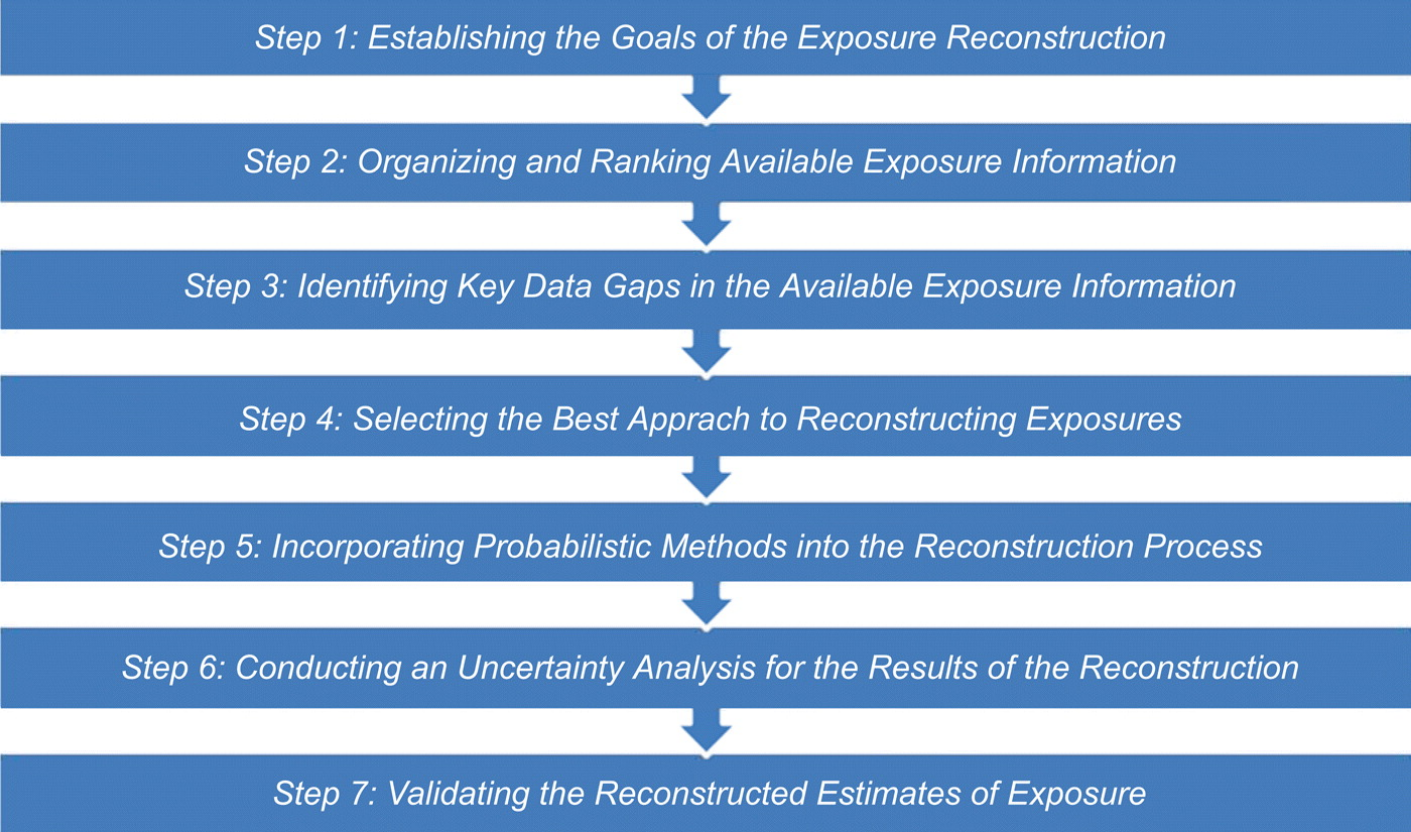
\includegraphics[width=0.5\textwidth,height=\textheight]{source/figures/ssframework.png}
\caption{Seven step framework for exposure
reconstruction\label{ssframework}}
\end{figure}

\hypertarget{job-exposure-matrices}{%
\paragraph{Job-exposure matrices}\label{job-exposure-matrices}}

Several job-exposure matrices that deal with asbestos have been
reported. Pannett et al's 1985 job-exposure matrix for use in population
studies in England and Wales{[}@Pannett1985{]} found good agreement
between job-title assigned categories of exposure (none, low, moderate,
high) for asbestos and direct review of the original occupational
history by an expert.

Rake et al{[}@Rake2009{]} assigned categories risk of exposure (low,
medium, high) using occupational mortality statistics for pleural
mesothelioma. Because pleural mesothelioma in men is nearly entirely
attributable to occupational asbestos exposure, pleural mesothelioma is
rapidly fatal, and UK death certificates record occupation in addition
to cause of death, the proportional mortality ratio for pleural
mesothelioma (standardised pleural mesothelioma mortality in a given
occupation/standardised pleural mesothelioma mortality across all
occupations) can serve as proxy for average asbestos exposure in a
particular occupation. This approach has been validated in the same
cohort by transmission electron microscopy asbestos fibre
counts.{[}@Gilham2016{]}

DOM-JEM{[}@Peters2011{]} was developed for use in a population based
multi-centre lung cancer case-control study conducted in seven european
countries. It assigns job titles one of three categories of asbestos
exposure (no exposure, low exposure, high exposure) based on the
consensus of three independent expert raters. DOM-JEM showed poor
agreement with expert assessment (\ensuremath{\kappa = 0.17}) but less
heterogeneity across countries than a population based JEM and expert
assessment. A study applying DOM-JEM to the Netherlands Cohort Study
(NCS) DOM-JEM also showed poor agreement with expert assessment (K =
0.29).{[}@Offermans2012{]}

The Finish Information System on Occupational Exposure
(FINJEM){[}@Kauppinen1998{]} covers exposure to 84 different agents,
including asbestos, for 311 jobs across 9 periods spanning 1945-2015.
Era-specific estimates of the mean level of asbestos exposure are
available for 27 jobs based on expert assessment and measurement data;
the exact details of the grounds for estimates are kept in a proprietary
FINJEM database which is sadly not freely available. FINJEM showed poor
agreement with expert assessment of asbestos exposure
(\ensuremath{\kappa = 0.23}) but reasonable identification of
mesothelioma risk when evaluated using the
NCS.{[}@Offermans2012{]}{[}@Offermans2014{]}

AsbJEM{[}@Oyen2015{]} was developed in Australia by an expert panel of
three industrial hygienists using all available exposure data. It is
based on FINJEM and provides quantitative estimates of annual exposure
for 224 occupations across three time periods spanning 1943 to 2004. It
also showed poor agreement with expert assessment of asbestos exposure
(\ensuremath{\kappa = 0.10}).{[}@Offermans2012{]}

SYN-JEM{[}@Peters2016{]} describes a JEM developed for four carcinogens.
It provides quantified asbestos exposure estimates based on 27958
personal measurements (spanning 1971-2009), a mixed effects statistical
model, and a priori categorical assessment of exposure (none, low,
high). Cherrie et al{[}@Cherrie2018{]} point out that SYN-JEM provides
little contrast in the modelled exposure level between categories as the
geometric mean for low jobs was 0.061 fibres/ml and for high jobs 0.074
fibres/ml and that there are wide variations in regional estimates that
are difficult to explain.

JEMS are generally taken to be superior to direct questions about
exposures because they are cheaper, have greater validity, and are less
vulnerable to differential recall. This is because recall of occupations
is not influenced by disease status, coding of occupation is blind to
case-control status, and translation of codes into exposure is
standardized and can not be influenced by disease status of a
subject.{[}@Ahrens1993{]}{[}@Teschke2002{]}{[}@Gramond2012{]}

Orlowski et al{[}@Orlowski1993{]} compared two JEMs with a structured
job specific questionnaire (SQ) in a lung cancer case-control study.
They found that agreement between the JEMs and the SQ was poor
(\ensuremath{\kappa = 0.23 to 0.27}) and suggested that the sources of
error for JEMs were loss of information due to the use of job codes as
surrogates for job task descriptions and the insufficiency of published
data on occupational asbestos exposure.

JEMs are not routinely used in clinical practice because they are not
usually available or accessible for specific patients. In a research
setting they are frequently helpful though in addition to the strengths
and weaknesses outlined above the desirability of reusing an existing
JEM vs developing a study specific JEM must be considered.

\hypertarget{exposure-modelling-approaches}{%
\paragraph{Exposure modelling
approaches}\label{exposure-modelling-approaches}}

Exposure modelling approaches modify existing measurement data on the
basis of knowledge of the determinants of exposure. They may be viewed
as the formalization of professional decision criteria used by
hygienists in their assessment of workplace exposures.{[}@Smith1991{]}

A common conceptual framework for this is the source-receptor
model{[}@Tielemans2008{]}{[}@Smith1991{]} whereby inhalation exposure is
considered in terms of an exposure source, a pathway from source to
receptor, and the receptor. The model is then used to propose modifying
factors such as activity emission potential, substance emission
potential, localized control, worker behavior, surface contamination and
respiratory protection.{[}@Tielemans2008{]}.

In the hands of some hygienists assessment of historic asbestos exposure
based on interview can correlate well with amphibole fibre
counts.{[}@Rodelsperger2001{]} By extension, exposure modelling
approaches, using industrial hygienist methods, might be expected to be
useful. Exposure modelling approaches make strong intuitive sense; it is
known that there is significant within-worker and between-worker
variability in occupational exposures{[}@Symanski2006{]} and, for
example, room size and ventilation have been empirically shown to affect
the concentration of airborne chemical exposures.{[}@Cherrie1999a{]}
Further, mathematical exposure models that take account of known
exposure modifying factors to estimate past exposures have shown a good
correlation with measured values.{[}@Cherrie1999{]}

A quantified validated historic asbestos exposure
model{[}@Cherrie2018{]} has recently been developed and proposed as a
means of for risk stratifying asbestos exposed workers to optimize
mesothelioma screening efforts. The approach has the advantage, compared
with job-exposure matrices, of providing a more granular quantified
exposure assessment, sensitive to the exposure circumstances of the
individual. However, the approach is limited by the fact that the
individual must recall their exposure circumstances which due to the
latency of asbestos related disease may have occurred over 30 years ago.
The approach is also limited by the relatively small number of
industry-specific data points used for validation, though though is
unavoidable because of the scarcity of exposure measurement data.

Exposure modelling approaches to assessing asbestos exposure have
research and clinical utility notwithstanding the limitations outlined
above together with the requirement that assessors be appropriately
trained.

\hypertarget{self-reported-exposure}{%
\paragraph{Self-reported exposure}\label{self-reported-exposure}}

Self-reported exposures are a subjects direct report of what they have
been exposed to. Typically this is elicited by asking about a specific
exposure via questionnaire or interview. Differential recall of
self-reported exposures according to disease status is a concern but few
studies have found evidence of this and it appears to be less of an
issue when prompted responses, rather than volunteered, responses about
occupational exposures are used.{[}@Teschke2000{]}

Most studies comparing self-reported exposures to industrial hygiene
measurements have found significant associations but with wide variation
in the proportions of variance explained by the self reports. This is
not surprising given that it is known there is significant within-worker
and between-worker variability in occupational
exposures.{[}@Teschke2002{]}{[}@Symanski2006{]}

Studies comparing self-reported exposures to expert assessment find
highly variable levels of agreement
(\ensuremath{\kappa = -0.05 to 0.94}) with a median
\ensuremath{\kappa = 0.6} . In two studies comparing self-reported
exposures with JEMs, self-reported exposures were more sensitive and of
similar or worse specificity.{[}@Teschke2002{]}

Self-reported exposures have been shown to be more accurate for easily
sensed exposures such as solvents with a strong smell, dusts with larger
particle sizes, and vibrations that can be felt. Providing a reference
point, for example using well known machines from a workplace to gauge
noise category also improves accuracy.{[}@Teschke2002{]}

Self-reported exposures have clinical utility in that they can suggest
or support consideration of an occupational cause for disease. Ideally
such self-reports are combined with the clinicians knowledge of the
likely occupational exposures given the occupational history and other
available data to strengthen or weaken the case as appropriate.
Similarly, they have utility in a research setting where they may
augment other means of assessment.

\hypertarget{discussion-2}{%
\subsection{Discussion}\label{discussion-2}}

The accuracy of historic asbestos exposure assessment, by any means, is
limited by the paucity of occupational asbestos measurement data,
measurement technique limitations, within and between worker exposure
variability, and participant recall. There does not exist a universally
agreed ``gold standard'' against which to evaluate methods. Accurate
quantified assessment of historic exposure, where evidence is scarce,
may be an impossible task.{[}@Burstyn2011{]}

Nonetheless, clinically, historic asbestos exposure assessments must be
made for attribution. Specifically, to inform whether the required
threshold of asbestos exposure (as assessed by various means) has been
crossed so it is possible to say that, for example, scarring of the lung
with an usual interstitial pneumonia pattern in an individual patient is
caused by asbestos exposure. This carries medicolegal in addition to
scientific importance and has not been well established by any
assessment method.

In the context of mesothelioma case-control studies fibre-counts do at
least provide an objective means of assessing historic asbestos exposure
against which other means can be compared. It is encouraging that
industrial hygienist assessment and assessment using job title and PMR
correlates strongly with fibre
counts.{[}@Gramond2012{]}{[}@Gilham2016{]} Further and more generally,
it is encouraging that estimates from explicit asbestos exposure
modelling systems such as Cherrie et al's{[}@Cherrie2018{]}, show good
correlation with measurement data.

\hypertarget{conclusion-2}{%
\subsection{Conclusion}\label{conclusion-2}}

Quantitative estimates of historic occupational asbestos exposures will
generally have high uncertainty. However, less precise measures, such as
relative difference in exposure among epidemiological groups may be
quite certain even though the numerical estimates are only approximate.
This is invaluable in studies examining aetiological
hypothesis.{[}@Smith1991{]}

\hypertarget{muc5b-environmental-insult-ipf}{%
\section{MUC5b + environmental insult =
IPF?}\label{muc5b-environmental-insult-ipf}}

\hypertarget{introduction-3}{%
\subsection{Introduction}\label{introduction-3}}

\hypertarget{mucus-mucins-muc5b-structure-function-and-evolutionary-importance}{%
\subsubsection{Mucus, Mucins, MUC5b: structure, function and
evolutionary
importance}\label{mucus-mucins-muc5b-structure-function-and-evolutionary-importance}}

Mucus is an essential part of the innate immune system, considered to be
universal within most phyla of both aquatic and terrestrial metazoans.
It plays a pivotal role in the prevention of disease by serving as an
antimicrobial barrier, it also has physiological functions including
allowing the exchange of oxygen, carbon dioxide, nutrient and
metabolites, lubricating surfaces and reducing damage due to sheer,
reducing dehydration of the epithelia and providing the polymeric matrix
which enables ciliary-mucus particle transport.

Mucus barriers are essential for the separation and protection of an
organism from its external environment, and likely a prerequisite for
the exclusion of bacteria from bodily tissues and evolution of
gastrointestinal and respiratory tracts. The importance of mucus
barriers is further underlined when one considers the energy investment
continuous mucus production and release requires; for example, corals
use mucus to trap particles and transport them towards their mouths and
the reef-building coral Acropora acuminata is thought to dedicate up to
40\% of its daily net carbon fixation (energy from photosynthesis) to
this task alone.{[}@Bakshani2018{]} Mucins are a key component of mucus,
they are highly evolutionary conserved large glycoproteins that date
back around 600 million years to Nematostella vectensis, the starlet sea
anemone, which is an early marine invertebrate. The earliest human mucin
analogue is found in Xenopus tropicalis, the African clawed frog, which
evolved about 300 million years ago and mucins are the likely
explanation for the observation that frogs show such great resistance to
infection during dissection and it has been shown that knockdown of
mucin in the skin mucus barrier of Xenopus tropicalis tadpoles leads to
susceptibility to infection by the opportunistic pathogen Aeromonas
hydrophila.{[}@Dubaissi2018{]}

The mucin family is composed of proteins that contain tandom repeat
structures with a high proportion of prolines, threonines, and serines;
the PTS domain. It is further defined by extensive glycosylation of the
PTS domain through N-Acetylgalactosamine O-linkages at the threonine and
serine residues.{[}@Kufe2009{]} The resultant oligisaccharide chains and
polymeric structure create the viscoeleastic properties of mucus which
confer its barrier properties and play an important role in storage and
secretion. {[}@Bakshani2018{]} Mucins are 50-90\% carbohydrate and they
are anionic because most of their terminal sugars contain carboxyl or
sulphate groups. Mucin glycan helps to sequester pathogen by acting as a
`decoy' and providing sites for microbial adhesins to bind; for example,
human salivary MUC5b interacts with streptococcal species, and patterns
of glycosylation change during
inflammation.{[}@Linden2008{]}{[}@Jaramillo2018{]} Mucin barriers can be
subverted by pathogens, strategies include production of enzymes to
degrade mucin core proteins and mucin carbohydrates, and evolution of
effective motility through mucus gels - many mucosal bacterial pathogens
are flagellated for this reason. There is evidence that degradative
enzymes are required for pathogenesis in species such as Vibrio cholorae
and that flagella are required for infectivity in species such as
Helicobacter pylori.{[}@Linden2008{]} Intracellular gel-forming mucins
are stored in a compact and condensed form in granules within
mucus-secreting cells. They are stored in solution with a high
concentration of calcium ions and protons which is thought to be
necessary to mask the anionic charge and prevent electrostatic
repulsion, upon secretion mucins expand 1000-3000 fold taking up water
to form a gel as calcium is exchanged for sodium and the pH
rises.{[}@Bakshani2018{]} One consequence of mucins being stored in such
a compact form is that when they're released they can obstruct the
airway which in mouse models appears necessary for the clearance of
helminth infection{[}@Jaramillo2018{]} and may provide a clue to their
evolution.

Normal human airway mucus is a hydrogel composed of approximately 98\%
water, 0.9\% salt, 0.8\% globular proteins, and 0.3\%
high-molecular-weight mucin polymers.{[}@Boucher2019{]} Mucin
hypersecretion may increase the concentration of solids up to 15\%
resulting in viscous elastic mucus that is not easily
cleared.{[}@Fahy2010{]} 17 genes encode mucins in the human genome of
which the gene products of seven are secreted and the remainder are
membrane bound. Five of the secreted mucins have terminal cysteine rich
domains that can form disulfide bonds resulting in polymers that impart
the properties of a gel. MUC5AC and MUC5B, two secreted gel-forming
mucins, are strongly expressed in the human respiratory tract. MUC5AC is
predominantly expressed in the conducting airways and MUC5B is
predominantly expressed in the respiratory airways (muc5b is also
expressed in salivary glands, cervix, gallbladder, seminal fluid, and
middle ear epithelium). Secreted mucins are large glycoproteins (up to
3x10\^{}6 D per monomer), ranking among the largest molecules encoded in
mammalian genomes, and their expression induces and requires an
endoplasmic reticulum stress response.{[}@Dickey2017{]} Mucin production
and secretion are regulated by distinct mechanisms. Production is highly
regulated at transcriptional level. The ErbB family of proteins contains
four receptor tyrosine kinases, structurally related to the epidermal
growth factor receptor (EGFR), its first discovered member.
ErbB-receptor signaling appears important for MUC5AC production since
inhibition blocks MUC5AC up-regulation by diverse stimuli.
Interleukin-13 (IL-13) is a cytokine secreted by T helper type 2 (Th2)
cells, CD4 cells, Natural killer T cell, Mast cell, Basophil cells,
Eosinophil cells and Nuocyte cells. IL-13 is a central regulator in IgE
synthesis, goblet cell hyperplasia, mucus hypersecretion, airway
hyperresponsiveness, fibrosis and chitinase up-regulation. It is a
mediator of allergic inflammation and different diseases including
asthma. IL-13 appears important because it increases MUC5AC expression
(IL-1 beta appears to be an important stimulus for MUC5b
expression{[}@Jaramillo2018{]}). Basal levels of production and
secretion of MUC5AC and MUC5B change as part of an allergic response.
The production of MUC5AC can increase 40-200 times as high as normal
levels in humans with similar findings in mice, MUC5B increases more
modestly, 3 to 10 times in mice. The most important stimulus for
secretion appears to be ATP which acts on apical membrane purinergenic
(P2Y\textsubscript{2}) receptors. Once secreted mucus gel is propelled
in a proximal direction towards the mouth, by ciliary beating as part of
the mucociliary escalator, where it is expectorated or swallowed.
{[}@Fahy2010{]}

\hypertarget{muc5b-rs3570950-and-respiratory-disease}{%
\subsubsection{MUC5b rs3570950 and respiratory
disease}\label{muc5b-rs3570950-and-respiratory-disease}}

Expression and localisation of MUC5AC and MUC5B is different in patients
with lung disease compared with healthy controls. MUC5AC expression is
increased in asthma for example, while MUC5B expression is increased in
COPD{[}@Kesimer2017{]} and IPF. In COPD MUC5b expression occurs in more
proximal airways, whereas in IPF it localised to the
bronchiole.{[}@Helling2017{]} MUC5b appears to be particularly important
in IPF.

The gain of function promoter variant rs5270590, 3.5 kb upstream of the
mucin 5b (MUC5B) transcriptional start site, is the strongest identified
risk factor (genetic or otherwise) for the development of either
sporadic or familial IPF. The largest study to date (1616 non- white
patients with fibrotic interstitial pneumonias and 4683 controls)
estimated that the odds of developing pulmonary fibrosis for those with
one copy of the risk allele were 4.5 times (95\% CI: 3.9, 5.2) the odds
of those with no copies and that the odds for those with two copies are
20.2 times those with no copies (95\% CI:
15.2--27.0).{[}@Fingerlin2013{]} The strength of association is
substantially higher than for most other common risk variants for
complex disease with the exception of the human leukocyte antigen (HLA)
region for some autoimmune diseases such as type-1 diabetes mellitus and
systemic lupus erythematosus which have OR greater than 10. The
association between rs35705950 has been replicated in 3 genome wide
association studies (GWAS) and a total of 10 independent cohorts
including a Mexican cohort and two Asian cohorts and is thought to
account for about a third of IPF cases.{[}@Evans2016{]} However,
penetrance is low with up to 20\% of non-Hispanic whites having at least
one copy of the variant yet IPF occurring only rarely (prevalence
\textless{} 1\%) . The rs35705950 variant is a G-to-T transversion that
occurs in an area of the MUC5B 5' flanking region, a region which has
characteristics of being an enhancer subject to epigenetic control via
DNA methylation and histone modification.{[}@Helling2017{]} An enhancer
is a sequence of DNA that functions to enhance transcription. A promoter
is a sequence of DNA that initiates the process of transcription. A
promoter has to be close to the gene that is being transcribed while an
enhancer does not need to be close to the gene of interest. Publicly
available data through the Encyclopedia of DNA Elements (ENCODE) suggest
MUC5b promoter site is a complex area of the genome with many
transcriptional factors showing evidence of binding.{[}@Selman2006{]} In
other words MUC5b expression likely a function of genetic and
non-genetic factors.{[}@Evans2016{]} In addition to IPF, rs35705950 has
been found to be positively associated with interstitial lung
abnormalities (ILA), chronic hypersensitivity pneumonitis (CHP),
rheumatoid arthritis associated interstitial lung disease (RA-ILD), and
myeloperoxidase-antineutrophil cytoplasmic antibody-associated
vasculitis associated interstitial lung disease
(AAV-ILD).{[}@Namba2019{]} It has also been found to not be associated
with cutaneous systemic sclerosis interstitial lung disease (SSc-ILD),
sarcoidosis, and myositis-ILD. {[}@Adegunsoye2019{]}

\hypertarget{potential-role-in-ipf-pathogenesis}{%
\paragraph{Potential role in IPF
pathogenesis}\label{potential-role-in-ipf-pathogenesis}}

The rs5270590 variant is associated with a 34 fold increase in
expression of MUC5b compared with wild type in healthy control
populations and a 5 fold increase in patients with IPF (see figure
1).{[}@Evans2016{]} In IPF patients distal airway MUC5b is expressed
preferentially, compared with MUC5Ac. MUC5b is also expressed in
honeycomb cysts, a defining characteristic of the usual interstitial
pneumonia CT pattern typically seen in IPF.{[}@Seibold2013{]}

\begin{figure}
\centering
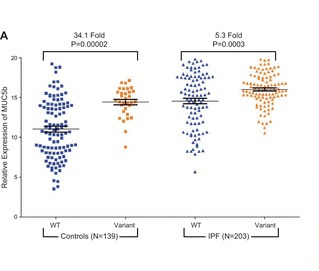
\includegraphics{source/figures/muc5b_expression.jpg}
\caption{MUC5b expression (Evans 2016)}
\end{figure}

Proposed mechanisms for the role of the rs5270590 variant in the
pathogenesis of IPF include:

\begin{enumerate}
\def\labelenumi{\arabic{enumi}.}
\tightlist
\item
  Excessive production of MUC5B by stem cells that attempt to regenerate
  injured bronchiolar and alveolar epithelium could disrupt normal
  development pathways and highjack normal reparative mechanisms of the
  distal lung resulting in fibroprolferation and honeycomb cyst
  formation.
\item
  Excessive MUC5B production leading to reduced mucociliary function,
  retention of particles, and enhanced lung injury.
\item
  Interaction between MUC5b and motile cilia since distinct cilium gene
  expression in IPF lung has been observed.
\item
  Excessive MUC5b production inducing endoplasmic reticulum stress and
  the unfolded protein response.{[}@Evans2016{]}
\end{enumerate}

Muc5b has been studied in mice. A muc5b knockout mouse study found that
muc5b is essential for mucociliary clearance, for controlling airway and
middle ear infections, and maintaining immune homeostasis in the lungs.
Knockout mice had airflow limitation and died from infection by multiple
bacterial species, including Staphylococcus aureus.{[}@Roy2014{]} A
transgenic muc5b mouse model of muc5b overexpression found that
overexpression causes mucociliary dysfuction and enhances lung fibrosis
on response to bleomycin.{[}@Hancock2018{]} Intriguingly, in recent
bleomycin lung fibrosis model studies lung fibrosis was attenuated and
mortality reduced in both germ-free mice and IL-17B deficient mice
supporting the concept that fibrosis in response to epithelial injury is
mediated by interaction of the immune system with
microbiota.{[}@ODwyer2019{]}{[}@Yang2019{]}

\hypertarget{infection-and-immunity}{%
\subsubsection{Infection and immunity}\label{infection-and-immunity}}

The frequency of the disease associated allele at rs35705950 exceeds
10\% in European populations
(https://www.ncbi.nlm.nih.gov/snp/rs35705950) but is less than 1\% in
African and East Asian populations. Clearly the rs35705950 variant is
not subject to negative selection due to IPF risk since onset is well
after the reproductive age begins{[}@Evans2016{]}; the variation in
frequency observed is consistent with strong positive selection. The
increased MUC5b expression in the airways associated with the rs35705950
variant may have conferred a survival advantage by providing protection
against lung infection. {[}@Dickey2017{]}{[}@Jaramillo2018{]} A relation
between the rs35705950 variant, disease risk, and infection is also
supported by the observation that in a prospective study of 65 IPF
patients and 44 COPD and health controls, IPF patients had higher
bacterial loads than COPD and healthy controls and within IPF patients
those with homozygous (TT) for variant had significantly lower bacterial
loads (P=0.01), measured by 16S rRNA quantitative polymerase chain
reaction of bronchoalveolar lavage samples. Within IPF those with higher
bacterial loads were also at increased risk of
death.{[}@Molyneaux2014{]} These finding are consistent with observation
that the rs35705950 variant is associated with improved survival in
IPF{[}@Peljto2013{]} and fewer acute respiratory disease events in the
COPDGene cohort with interstitial features.{[}@Ash2018{]} However, these
studies are vulnerable to index event bias, by which selection of
subjects according to disease status creates biased associations if
common causes of incidence and prognosis if not properly accounted
for.{[}@Dudbridge2019{]} For example, it is known that the rs35705950
variant is associated with interstitial lung
abnormalities{[}@Hunninghake2013{]}, since the diagnosis of IPF relies
heavily on radiological appearances individuals with the variant might
tend to be diagnosed earlier in the course of their disease giving the
false impression, when comparing them to IPF patients without the
disease variant that is associated with survival. Further support for
the importance of infection in IPF provided by the observation that
immunomodulatory therapies such as interferon gamma, ethanercept,
prednisolone, azathioprine and N-acetylcysteine have failed to prolong
survival in IPF{[}@WarheitNiemi2019{]} to prolong survival in IPF, from
a small (N = 181) double blinded randomized controlled study which found
reduced symptom burden and improved survival associated with
cotrimoxazole{[}@Shulgina2013{]}, as well as evidence from genetic and
animal studies. IPF GWAS have identified single nucleotide variants
associated with disease susceptibility in the Toll interacting protein
(TOLLIP) gene, for example rs111521887. TOLLIP is an inhibitory adaptor
protein within Toll-like receptors (TLR) and part of the innate immune
system recognising pathogen associated molecular patterns
(PAMPs){[}@Noth2013{]} and, intriguingly, in a mouse bleomycin lung
fibrosis model the absence of a microbiome protected against
mortality.{[}@ODwyer2019{]}

\hypertarget{inorganic-occupational-stimuli}{%
\subsubsection{Inorganic occupational
stimuli}\label{inorganic-occupational-stimuli}}

The frequency of the disease associated allele at rs35705950 exceeds
10\% in European
populations(https://www.ncbi.nlm.nih.gov/snp/rs35705950) but its
penetrance is low; the median prevalence of IPF for men and women in
Europe is approximately 3.75 per 100000 for the period
2001-2013{[}@Marshall2018{]}, which suggests other genetic or
environmental factors must be at play. In addition to responding to
PAMPs as outlined above the innate immune system also responds to
damage-associated molecular patterns (DAMPs) which can result from
inhalation of inorganic respirable toxins such as silica or
asbestos.{[}@Dostert2008{]} Secretion of the inflammatory cytokine IL-1
beta) (which is also a stimulus for MUC5b expression) is elevated in
alveolar macrophages of patients with ILD, including IPF, sarcoidosis,
silicosis, RA-ILD, and asbestosis.{[}@Byrne2016{]}{[}@Howrylak2017{]}
Inflammasome are multiprotein intracellular complexes that detect
pathogenic microorganisms (PAMPs) and sterile stressors (DAMPs). The
NLRP3 (NOD-, LRR- and pyrin domain-containing protein 3) inflammasome is
an intracellular sensor that detects a broad range of PAMPs and DAMPs
leading to caspase 1-dependent release of the pro-inflammatory cytokines
IL-1 beta and IL-18, as well as to gasdermin D-mediated pyroptotic cell
death.{[}@Swanson2019{]} Interestingly the NLRP3 inflammasome appears to
be implicated, albeit with differing activation
patterns{[}@Lasithiotaki2016{]}, in all of these conditions, interaction
between smoking (a risk factor for IPF) and the NLRP3 inflammasome is
recognised, and recent work has shown age-dependent susceptibility to
pulmonary fibrosis in a bleomycin-induced lung injury mouse
model.{[}@StoutDelgado2016{]} Occupational risk factors such as metal,
wood, and stone dust exposure are well recognised in IPF, accounting for
up to 8\% of cases the basis of a meta-analysis of case-control
data{[}@Blanc2019{]} and its likely that innate immune system activation
via the NLRP3 inflammasome and other means by occupational exposures
mediates this risk.

\hypertarget{conclusion-3}{%
\subsection{Conclusion}\label{conclusion-3}}

The apparently complex interplay between exposure to organic and
inorganic respiratory toxins, the mucus barrier, respiratory epithelium
and resident cells such as alveolar macrophages in idiopathic pulmonary
fibrosis remains incompletely characterised but genetic, epigenetic,
gene-expression, and epidemiological studies are beginning to fill in
the gaps. Gene-environment interaction between the rs5270590 variant and
occupational inorganic respiratory toxins such as asbestos may modulate
IPF risk and help to explain the incomplete penetrance observed. Studies
to date which have selected patients on the basis of a diagnosis of IPF
and then stratified by MUC5b genotype are at risk of index-event bias. A
large case-control study of IPF which captures details of occupational
exposures, genotype, and potential confounders, whilst also measuring
factors likely to affect disease pickup such as disease severity and
radiographic changes is required.

\hypertarget{idiopathic-pulmonary-fibrosis-job-exposures-study-ipfjes-is-occupational-asbestos-exposure-an-under-recognised-cause-of-ipf}{%
\section{Idiopathic pulmonary fibrosis job exposures study (IPFJES): Is
occupational asbestos exposure an under-recognised cause of
IPF?}\label{idiopathic-pulmonary-fibrosis-job-exposures-study-ipfjes-is-occupational-asbestos-exposure-an-under-recognised-cause-of-ipf}}

\hypertarget{introduction-4}{%
\subsection{Introduction}\label{introduction-4}}

Occult occupational asbestos exposure as a cause for otherwise
`idiopathic' pulmonary fibrosis has been an open question for at least
30 years. The question arises because of the clinical and radiological
similarities of asbestosis and IPF; a usual interstitial pneumonia is
observed in both, and patients can present in the same way (chapter 1).
Patients having significant asbestos exposure, that would warrant a
diagnosis of asbestosis, may go undetected because they do not recall
exposure or because where they do recall exposure it is difficult to
assess if the exposure is sufficient to have caused disease (chapter 4).
A recent meta-analysis of IPF case control studies reporting on
occupational exposures found significant associations between metal,
wood, and stone dust, and IPF (chapter 2). However, the extent of
confounding by groups of workers likely to have significant asbestos
co-exposure, for example carpenters and metal plate workers, is unknown.
The majority of these studies are limited by their reliance on
self-reported binary exposure which risks recall bias and does not
permit investigation of dose-response relationships which would be
helpful for establishing causality. Studies to date have also not looked
at the possibility of gene-environment interaction; genetic risk factors
such as rs5270590 are now well established and interaction with inhaled
exposures is suspected but has not yet proven in humans (chapter 5). The
question of asbestos exposure in IPF is a live one globally because
countries such as Brazil, Russia, India, and China, continue to consume
asbestos and, closer to home, asbestos related and IPF mortality rates
continue to rise; asbestos related mortality in the UK is driven
primarily by pleural mesothelioma and is expected to peak in the next
couple of years as a result of effective asbestos exposure control
legislation, the sustained rise in IPF mortality rates is unexplained
(chapter 3).

IPFJES is a multi-centre, hospital-outpatient, incident case-control
study conceived to definitively address the question of asbestos
exposure having a causal role in IPF. Participants were recruited from a
network of 21 hospitals across England, Scotland, and Wales. Cases were
men who presented, between 01/02/2017 and 01/10/2019, with a new MDT
diagnosis of IPF consistent with standard criteria.{[}@Raghu2011{]}
Controls were men who attended selected outpatient clinics in the same
time period. An outpatient clinic was randomly selected to be the source
clinic for the recruitment of controls at each hospital from a list of
all outpatient clinics (not confined to respiratory) local research
teams could recruit from. Over 460 cases and 460 controls,
frequency-matched on age, were recruited to achieve a pre-defined
recruitment target of 920 participants.{[}clinicaltrials.gov
NCT03211507{]} Participants were interviewed by telephone by a trained
interviewer who was blind to their case status using a bespoke study web
application (ipfjes-interview, full source code available at
www.ipfjes.org). Lifetime occupational history, smoking history, drug
history, family history, and modified Medical Research Council (mMRC)
dyspnoea score were recorded. Using ipfjes-interview each occupation was
coded on the basis of the Office for national statistics (ONS)
standardised occupational classification 1990 (SOC90) at the time of the
interview. For participants who recalled carrying out work tasks with
asbestos a detailed assessment of each work task was recorded. SOC90
coded jobs were used to assign asbestos exposure risk to participants
using occupational proportional mortality rates for malignant pleural
mesothelioma. A fibre-ml.year estimate was calculated for participants
recalling asbestos exposure. All participants provided an EDTA sample
from which DNA was extracted and genotyped according to IPF
susceptibility single nucleotide variant (SNV) rs35705950 using Q-PCR
and a Taqman assay. Unconditional logistic regression was used to
analyse `any' vs `no' asbestos exposure and categories of cumulative
exposure adjusting for age and smoking status. In a secondary analysis
we used logistic regression to investigate metal, wood, and stone dust
exposure (self-reported occupational exposure), and rs35705950
genotype-exposure interactions.

\hypertarget{method-3}{%
\subsection{Method}\label{method-3}}

\hypertarget{funding-approvals-and-registration}{%
\subsubsection{Funding, approvals, and
registration}\label{funding-approvals-and-registration}}

We obtained funding from welcome trust (201291/Z/16/Z) and ethical
approval (IRAS project ID 203355, REC reference 17/EM/0021). We also
obtained NIHR portfolio status (CPMS ID 203355) and registered our study
on clinicaltrials.gov (NCT03211507). Full study documentation is
available online at www.ipfjes.org.

\hypertarget{selection}{%
\subsubsection{Selection}\label{selection}}

Cases were men of any age who were diagnosed with IPF at 21
collaborating hospitals across England, Scotland, and Wales between
01/02/2017 and 01/10/2019. The diagnosis of IPF by the referring centres
was made at MDT on the basis of clinical history, high-resolution
computed-tomography (HRCT), and where necessary lung biopsy in
accordance with standard criteria.{[}@Raghu2011{]} Referring centres
provided HRCT report findings for all cases and histopathology report
findings for cases where a biopsy was performed.

At each collaborating hospital an outpatient clinic was randomly
selected to be the source clinic for the recruitment of controls from a
list of all outpatient clinics (not confined to respiratory) that the
local research team could recruit. If the clinic selected was
unsuitable, for example because it did not contain men of a similar age
to cases or the clinic lead declined to participate then this was
recorded and a further random selection made. Controls were men that
attended the selected outpatient clinics between 01/02/2017 and
01/10/2019. Controls were frequency-matched on age, were recruited to
achieve a pre-defined recruitment target of 920 participants.

Men who were unable to give informed consent or who had worked outside
of the UK for one year or more (not including work outside the UK by a
member of the armed forces or merchant navy) were excluded from being
cases and controls. Cases and controls were approached by local research
teams and provided with the IPFJES participant information sheet. They
were given opportunity to read it and ask questions and then invited to
sign the consent form and provide their contact details and a blood
sample if they wished to take part. Local researchers completed a case
report form detailing participant demographic information, CT and biopsy
results, and contact details which was sent together with the blood
sample by secure post to the central research team.

\hypertarget{measures}{%
\subsubsection{Measures}\label{measures}}

A trained interviewer (RS or CR) who was blind to the case status of
participants conducted the study interviews by telephone. Interviews
were recorded for quality control purposes. The interviewer used a
bespoke web application, called ipfjes-interview, to administer a
structured interview collecting information on lifetime occupational
history, smoking history, drug history, family history, mMRC dyspnoea
score, comorbidities, and presenting symptoms. For each job information
was collected on the job title, job tasks, employer, start and stop year
of employment, and whether employment was full-time (\textgreater=35
hour per week) or part time. Smoking history was recorded as start and
stop year of smoking, number of cigarettes (or equivalent using
https://www.smokingpackyears.com/) per day, and what was smoked -
cigarettes/roll-ups/pipe/other. Participants were asked about prior
exposure to nine drugs suspected of causing usual interstitial pneumonia
(amiodarone, azathioprine, bleomycin, flecainide, gefitinib, ifosamide,
melphalan, and nitrofurantoin).{[}@Bonniaud2014{]} Using the job title
and ipfjes-interview each occupation was coded in real time to the
office for national statistics (ONS) standardised occupational
classification 1990 (SOC90).

SOC90 coded jobs were used to assign asbestos exposure risk to
participants using occupational proportional mortality rates for
malignant pleural mesothelioma{[}@Peto2009{]}. For participants who
recalled carrying out work tasks with asbestos a detailed assessment of
each work task was recorded. A fibre-ml/year estimate was calculated
using a model with parameters for the type of asbestos used (substance
emission potential, E), what was done with it (activity emission
potential, H), how well ventilated the room the activity was carried out
in was (general ventilation parameters, D), and whether there were any
local exposure controls, for example wetting (local controls, LC). The
calculation to estimate asbestos exposure (AE) for a given asbestos
related task was: AE = E * H * LC. AE for each task was then weighted
according to the amount total of time spent performing the task arrive
at a task fibre-ml/year exposure estimate. Task fibre-ml/year exposure
estimates were then summed at an individual participant level to provide
an overall fibre-ml/year estimate. A random sample of high (top 25\% of
values), medium (25-75\% centile), and low (bottom 25\% of values)
estimates was checked by a hygiene assessment expert who was blind to
participant case status (JC).{[}@Cherrie1999{]}{[}@Cherrie2018{]}

SOC90 coded jobs were also used to assign National Statistics
Socio-economic analytic classes (NS-SEC). The Office of National
Statistics provides a lookup to assign each SOC90 code to one of eight
classes:

\begin{enumerate}
\def\labelenumi{\arabic{enumi}.}
\tightlist
\item
  Higher managerial, administrative and professional occupations. 1.1
  Large employers and higher managerial and administrative occupations.
  1.2 Higher professional occupations.
\item
  Lower managerial, administrative and professional occupations
\item
  Intermediate occupations
\item
  Small employers and own account workers
\item
  Lower supervisory and technical occupations
\item
  Semi-routine occupations
\item
  Routine occupations
\item
  Never worked and long-term unemployed
\end{enumerate}

We then assigned each individual to a single code by calculating the
median code for all of the jobs they had held.

Participants were classified as occupationally exposed to stone, wood,
and metal dust or not (binary measure) on the basis of the recorded
participant provided description of tasks carried out within a job
including the words `stone' (or `silica'), `wood', or `metal',
respectively.

All participants provided an EDTA sample from which DNA was extracted
and genotyped according to IPF susceptibility single nucleotide variant
(SNV) rs35705950. DNA was extracted using a nucleon dna extraction kit
(protocol). Genotypes of the MUC5B SNP rs35705950 were determined using
TaqMan assays (Life Technologies, Carlsbad, CA). Reactions were
performed in 96-well plates, and fluorescence was read using an Applied
Biosystems Viia7 Sequence Detection System.

\hypertarget{statistical-analysis}{%
\subsubsection{Statistical analysis}\label{statistical-analysis}}

Unconditional logistic regression was used to analyse `any' vs `no'
asbestos exposure and categories of cumulative exposure adjusting for
age, smoking status and recruiting centre as part of a prespecified
analysis (clinicaltrials.gov NCT03211507).

In an unplanned secondary analysis we used logistic regression to
investigate metal, wood, and stone dust exposure (self-reported
occupational exposure), and rs35705950 genotype-exposure interactions.
Sensitivity analysis of distance to centre was also performed because we
expected cases to live further away from the hospital that controls on
average (as IPF care is centralised to a select number of specialist
centres) and we hypothesised that distance from the hospital might be
associated with likelihood of exposure to asbestos. We used Pearson's
correlation coefficient to investigate associations between individual
variables, such as distance from hospital and fibre-ml.year asbestos
exposure estimates. We used ordinal logistic regression to investigate
the relationship between mMRC dyspnoea score and measures of asbestos
exposure.

\hypertarget{results-3}{%
\subsection{Results}\label{results-3}}

516 cases and 511 controls were recruited to IPFJES in the study period
Feb 2017 to October 2019. 22 of 516 cases(4\%), and 45 of 511
controls(9\%) were withdrawn because they no longer wished to take part
in the study, they did not respond after we called them on three
occasions, or we were notified that they had died before the interview
took place. The remaining 960 participants (494 cases, 466 controls)
comprise the study sample.

The median year of birth and age was 1943 and 76 for cases and 1945 and
74 for controls. Most cases and controls reported their ethnicity as
white (97\% and 96\% respectively). Social economic class and exposure
to smoking were similar for cases and controls (see Table one).

\newpage

\hypertarget{table-one-participant-demographic-characteristics}{%
\subsubsection{Table one: Participant demographic
characteristics}\label{table-one-participant-demographic-characteristics}}

\begin{longtable}[]{@{}lllll@{}}
\toprule
Characteristic & Cases (N=494) & \% & Controls (N=466) &
\%\tabularnewline
\midrule
\endhead
Age -- yr & & & &\tabularnewline
median & 76 & & 74 &\tabularnewline
interquartile range & 71-81 & & 69-79 &\tabularnewline
& & & &\tabularnewline
Ethnicity & & & &\tabularnewline
White & 479 & 97 & 449 & 96\tabularnewline
Asian/Asian British & 11 & 2 & 8 & 2\tabularnewline
Black/African & 2 & 0 & 7 & 2\tabularnewline
Mixed/Other & 2 & 0 & 2 & 0\tabularnewline
& & & &\tabularnewline
Social class & & & &\tabularnewline
1.1 & 2 & 0 & 11 & 2\tabularnewline
1.2 & 33 & 7 & 28 & 6\tabularnewline
2 & 58 & 12 & 63 & 14\tabularnewline
3 & 73 & 15 & 71 & 15\tabularnewline
4 & 53 & 11 & 50 & 11\tabularnewline
5 & 92 & 19 & 100 & 21\tabularnewline
6 & 117 & 24 & 87 & 19\tabularnewline
7 & 66 & 13 & 56 & 12\tabularnewline
& & & &\tabularnewline
Smoking & & & &\tabularnewline
Current smoker & 10 & 2 & 30 & 6\tabularnewline
Ever smoked & 373 & 76 & 327 & 70\tabularnewline
Packyears & & & &\tabularnewline
mean & 27 & & 24 &\tabularnewline
median & 20 & & 19 &\tabularnewline
interquartile range & 9-36 & & 7-34 &\tabularnewline
\bottomrule
\end{longtable}

All cases had a CT thorax and this was reported as definite UIP in 266
(54\%) cases, possible UIP in 216 (44\%) cases, or other 12 (2\%) cases.
Nine cases (2\%) had a biopsy because the CT was thorax was
non-diagnostic, all of these were reported as define UIP. Cases were
more breathless than controls as measured by the Medical Research
Council (MRC) dyspnoea scale and known rs3570950 IPF associations were
evident (see Table two).

\hypertarget{table-two-patient-clinical-features-from-case-report-form-and-genotypes}{%
\subsubsection{Table two: Patient clinical features (from case report
form) and
genotypes}\label{table-two-patient-clinical-features-from-case-report-form-and-genotypes}}

\begin{longtable}[]{@{}lllll@{}}
\toprule
& Cases (N=494) & \% & Controls (N=466) & \%\tabularnewline
\midrule
\endhead
CT & & & &\tabularnewline
no CT & 0 & 0 & 462 & 99\tabularnewline
definite UIP & 266 & 54 & 1\textsuperscript{1} & 0\tabularnewline
possible UIP & 216 & 44 & 0 & 0\tabularnewline
other & 12 & 2 & 3 & 1\tabularnewline
& & & &\tabularnewline
Bx & & & &\tabularnewline
no biopsy & 485 & 98 & 466 & 100\tabularnewline
definite UIP & 9 & 2 & 0 & 0\tabularnewline
& & & &\tabularnewline
mMRC & & & &\tabularnewline
0 & 35 & 7 & 254 & 55\tabularnewline
1 & 94 & 19 & 65 & 14\tabularnewline
2 & 165 & 33 & 80 & 17\tabularnewline
3 & 172 & 35 & 65 & 14\tabularnewline
4 & 28 & 6 & 2 & 0\tabularnewline
& & & &\tabularnewline
rs35705950 genotype & N=395 & & N=423 &\tabularnewline
(G;G) & 212 & 54 & 327 & 77\tabularnewline
(G;T) & 152 & 38 & 91 & 22\tabularnewline
(T;T) & 31 & 8 & 5 & 1\tabularnewline
\bottomrule
\end{longtable}

\textsuperscript{1} one control had rheumatoid arthritis associated
interstitial lung disease

Randomly-selected control clinics for recruiting centres are shown in
Table three. Where more than one clinic is shown this indicates that the
random selection process was repeated because of difficulty recruiting
adequate numbers of participants (defined as four attendances to the
control clinic by the local research team and fewer than four
participants recruited).

\newpage

\hypertarget{table-three-centre-control-clinic-and-recruitment}{%
\subsubsection{Table three: centre control clinic and
recruitment}\label{table-three-centre-control-clinic-and-recruitment}}

\begin{longtable}[]{@{}lll@{}}
\toprule
& Cases (N=494) & Controls (N=466)\tabularnewline
\midrule
\endhead
centre number (control source clinic) & &\tabularnewline
1 (General Surgery) & 42 & 39\tabularnewline
2 (Gastroenterology/Stroke) & 13 & 11\tabularnewline
3 (Cardiology) & 38 & 36\tabularnewline
4 (Urology) & 52 & 52\tabularnewline
5 (Diabetes/Rheumatology) & 40 & 31\tabularnewline
6 (Sleep Apnea) & 34 & 37\tabularnewline
7 (Neurology) & 15 & 16\tabularnewline
8 (ENT) & 40 & 39\tabularnewline
9 (Rheumatology) & 31 & 29\tabularnewline
10 (Oncology) & 21 & 73\textsuperscript{1}\tabularnewline
11 (Urology) & 11 & 11\tabularnewline
12 (Haematology) & 4 & 3\tabularnewline
13 (Respiratory) & 13 & 14\tabularnewline
14 (Cardiology) & 20 & 16\tabularnewline
15 (Cardiology) & 15 & 14\tabularnewline
16 (Orthopaedics) & 39 & 2\textsuperscript{2}\tabularnewline
17 (Asthma) & 6 & 6\tabularnewline
18 (Hypertension) & 15 & 1\textsuperscript{2}\tabularnewline
19 (General Surgery) & 7 & 9\tabularnewline
20 (Urology) & 31 & 25\tabularnewline
21 (Respiratory) & 7 & 2\tabularnewline
\bottomrule
\end{longtable}

\textsuperscript{1} Controls were over-recruited at the local
participating centre to help to achieve the recruitment target.
\textsuperscript{2} Controls were under-recruited because of local
research staffing shortage.

330 (67\%) cases and 295 (63\%) controls ever had a high or medium
asbestos exposure risk job, defined on the basis of proportional
occupational mortality statistics.{[}@Peto2009{]} Ever having a high or
medium asbestos exposure risk job was not associated with IPF (see Table
four).

\hypertarget{table-four-occupational-asbestos-exposure-inferred-by-job-title-and-ipf-risk-ever-vs-never}{%
\subsubsection{Table four: Occupational asbestos exposure (inferred by
job title) and IPF risk (ever vs
never)}\label{table-four-occupational-asbestos-exposure-inferred-by-job-title-and-ipf-risk-ever-vs-never}}

\begin{longtable}[]{@{}lllll@{}}
\toprule
\begin{minipage}[b]{0.06\columnwidth}\raggedright
\strut
\end{minipage} & \begin{minipage}[b]{0.10\columnwidth}\raggedright
Cases (\%)\strut
\end{minipage} & \begin{minipage}[b]{0.12\columnwidth}\raggedright
Controls (\%)\strut
\end{minipage} & \begin{minipage}[b]{0.29\columnwidth}\raggedright
Unadjusted OR (95\%CI; p-value)\strut
\end{minipage} & \begin{minipage}[b]{0.28\columnwidth}\raggedright
Adjusted OR\textsuperscript{1} (95\%CI; p-value)\strut
\end{minipage}\tabularnewline
\midrule
\endhead
\begin{minipage}[t]{0.06\columnwidth}\raggedright
ever\strut
\end{minipage} & \begin{minipage}[t]{0.10\columnwidth}\raggedright
330(67)\strut
\end{minipage} & \begin{minipage}[t]{0.12\columnwidth}\raggedright
295(63)\strut
\end{minipage} & \begin{minipage}[t]{0.29\columnwidth}\raggedright
1.17(0.9-1.5; 0.28)\strut
\end{minipage} & \begin{minipage}[t]{0.28\columnwidth}\raggedright
1.09(0.8-1.5; 0.6)\strut
\end{minipage}\tabularnewline
\begin{minipage}[t]{0.06\columnwidth}\raggedright
never\strut
\end{minipage} & \begin{minipage}[t]{0.10\columnwidth}\raggedright
164(33)\strut
\end{minipage} & \begin{minipage}[t]{0.12\columnwidth}\raggedright
171(37)\strut
\end{minipage} & \begin{minipage}[t]{0.29\columnwidth}\raggedright
1\strut
\end{minipage} & \begin{minipage}[t]{0.28\columnwidth}\raggedright
1\strut
\end{minipage}\tabularnewline
\bottomrule
\end{longtable}

\textsuperscript{1} Adjusted for age, smoking, and centre

There was a non-statistically significant trend in the unadjusted OR
whereby higher exposure categories had higher (non-significant) OR for
disease (see Table five). Chi\textsuperscript{2} test for trend was 1.7,
p=0.19.

\newpage

\hypertarget{table-five-occupational-asbestos-exposure-inferred-by-job-title-and-ipf-risk-categories-of-exposure}{%
\subsubsection{Table five: Occupational asbestos exposure (inferred by
job title) and IPF risk (categories of
exposure)}\label{table-five-occupational-asbestos-exposure-inferred-by-job-title-and-ipf-risk-categories-of-exposure}}

\begin{longtable}[]{@{}lllll@{}}
\toprule
\begin{minipage}[b]{0.20\columnwidth}\raggedright
Category\strut
\end{minipage} & \begin{minipage}[b]{0.08\columnwidth}\raggedright
Cases (\%)\strut
\end{minipage} & \begin{minipage}[b]{0.10\columnwidth}\raggedright
Controls (\%)\strut
\end{minipage} & \begin{minipage}[b]{0.24\columnwidth}\raggedright
Unadjusted OR (95\%CI; p-value)\strut
\end{minipage} & \begin{minipage}[b]{0.23\columnwidth}\raggedright
Adjusted OR\textsuperscript{1} (95\%CI; p-value)\strut
\end{minipage}\tabularnewline
\midrule
\endhead
\begin{minipage}[t]{0.20\columnwidth}\raggedright
high-risk non-construction\strut
\end{minipage} & \begin{minipage}[t]{0.08\columnwidth}\raggedright
65(13)\strut
\end{minipage} & \begin{minipage}[t]{0.10\columnwidth}\raggedright
52(11)\strut
\end{minipage} & \begin{minipage}[t]{0.24\columnwidth}\raggedright
1.30(0.8-2.1;0.3)\strut
\end{minipage} & \begin{minipage}[t]{0.23\columnwidth}\raggedright
1.10(0.7-1.8; 0.7)\strut
\end{minipage}\tabularnewline
\begin{minipage}[t]{0.20\columnwidth}\raggedright
high-risk construction\strut
\end{minipage} & \begin{minipage}[t]{0.08\columnwidth}\raggedright
141(29)\strut
\end{minipage} & \begin{minipage}[t]{0.10\columnwidth}\raggedright
126(27)\strut
\end{minipage} & \begin{minipage}[t]{0.24\columnwidth}\raggedright
1.17(0.8-1.8;0.5)\strut
\end{minipage} & \begin{minipage}[t]{0.23\columnwidth}\raggedright
1.13(0.8-1.7; 0.55)\strut
\end{minipage}\tabularnewline
\begin{minipage}[t]{0.20\columnwidth}\raggedright
medium risk industrial\strut
\end{minipage} & \begin{minipage}[t]{0.08\columnwidth}\raggedright
124(25)\strut
\end{minipage} & \begin{minipage}[t]{0.10\columnwidth}\raggedright
117(25)\strut
\end{minipage} & \begin{minipage}[t]{0.24\columnwidth}\raggedright
1.11(0.7-1.7;0.64)\strut
\end{minipage} & \begin{minipage}[t]{0.23\columnwidth}\raggedright
1.06(0.7-1.6; 0.79)\strut
\end{minipage}\tabularnewline
\begin{minipage}[t]{0.20\columnwidth}\raggedright
low risk industrial\strut
\end{minipage} & \begin{minipage}[t]{0.08\columnwidth}\raggedright
94(19)\strut
\end{minipage} & \begin{minipage}[t]{0.10\columnwidth}\raggedright
98(21)\strut
\end{minipage} & \begin{minipage}[t]{0.24\columnwidth}\raggedright
1(0.7-1.5;0.99)\strut
\end{minipage} & \begin{minipage}[t]{0.23\columnwidth}\raggedright
0.94(0.6-1.5; 0.78)\strut
\end{minipage}\tabularnewline
\begin{minipage}[t]{0.20\columnwidth}\raggedright
office\strut
\end{minipage} & \begin{minipage}[t]{0.08\columnwidth}\raggedright
70(14)\strut
\end{minipage} & \begin{minipage}[t]{0.10\columnwidth}\raggedright
73(16)\strut
\end{minipage} & \begin{minipage}[t]{0.24\columnwidth}\raggedright
1\strut
\end{minipage} & \begin{minipage}[t]{0.23\columnwidth}\raggedright
1\strut
\end{minipage}\tabularnewline
\bottomrule
\end{longtable}

\textsuperscript{1} Adjusted for age, smoking, and centre

A total of 463 asbestos exposed job tasks were recalled in sufficient
detail to permit a fibre-ml.year estimate of exposure by 233 individual
participants. 125 (25\%) of cases and 108 (23\%) of controls recalled
occupational asbestos exposure in sufficient detail to permit estimation
of cumulative fibre-ml.year exposure. 41 (33\%) of cases and 35 (32\%)
of controls which equated to approximately 8\% of the total number of
cases and 8\% of the total number of controls, had cumulative estimates
exceeding 25 asbestos fibre-ml.years (see Table six).

\newpage

\hypertarget{table-six-occupational-asbestos-exposure-cumulative-fibre-ml-year-estimate-and-ipf-risk}{%
\subsubsection{Table six: Occupational asbestos exposure (cumulative
fibre ml year estimate) and IPF
risk}\label{table-six-occupational-asbestos-exposure-cumulative-fibre-ml-year-estimate-and-ipf-risk}}

\begin{longtable}[]{@{}lllllllll@{}}
\toprule
& N (\% total) & median & 0-4 & 5-9 & 10-14 & 15-19 & 20-24 &
\textgreater{} 25\tabularnewline
\midrule
\endhead
cases & 125 (25) & 6.86 & 62 (50) & 10 (8) & 8 (6) & 3 (2) & 4 (3) & 41
(33)\tabularnewline
controls & 108 (23) & 4.36 & 56 (52) & 4 (4) & 5 (5) & 0 (0) & 5 (5) &
35 (32)\tabularnewline
\bottomrule
\end{longtable}

Fibre-ml.year exposure assessments showed reasonable correlation on the
log-scale, but not the linear scale, with an independent assessor (JC)
for a validation sample of low, medium, and high exposure assessments,
R\textsuperscript{2} = 0.63 (see Figures 6.1).

\begin{figure}
\centering
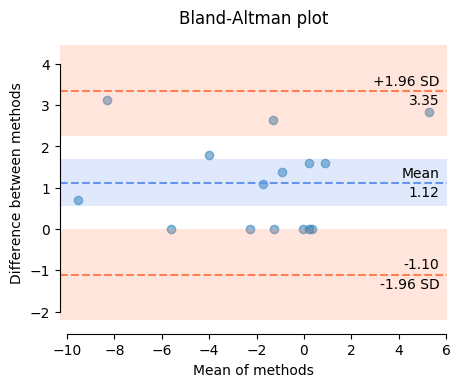
\includegraphics[width=0.5\textwidth,height=\textheight]{source/figures/cherrie_validation.png}
\caption{Independent validation of fibre-ml.year exposure assessments}
\end{figure}

108(23\%) of 463 asbestos exposed job task fibre-ml.year estimates were
in excess of 25 fibre-ml.years. 81(75\%) occurred in jobs classified as
high risk or medium risk; 17(15\%) occurred in high-risk
non-construction jobs e.g boiler lagger, 54(50\%) in high-risk
construction jobs such as carpenter, electrician, and plumber, and 10
(9\%) in medium risk industrial jobs such as machinist or fitter.
Carpenter was the single most common job title accounting for 6(5\%) of
estimates in excess of 25 fibre-ml.years (see Figures 6.2 and 6.3).

\begin{figure}
\centering
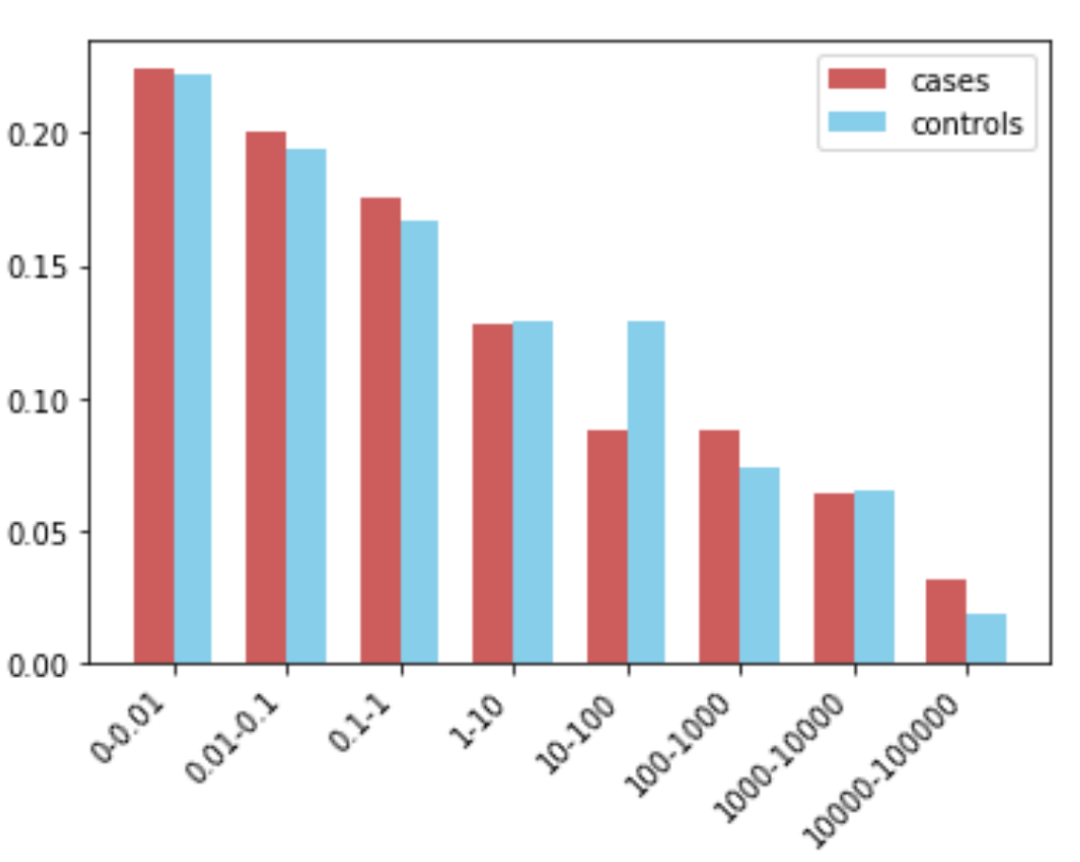
\includegraphics[width=0.5\textwidth,height=\textheight]{source/figures/fibre.png}
\caption{Proportion of exposed participants in fibre-ml.year categories
of exposure for those reporting exposure (N=108)}
\end{figure}

\begin{figure}
\centering
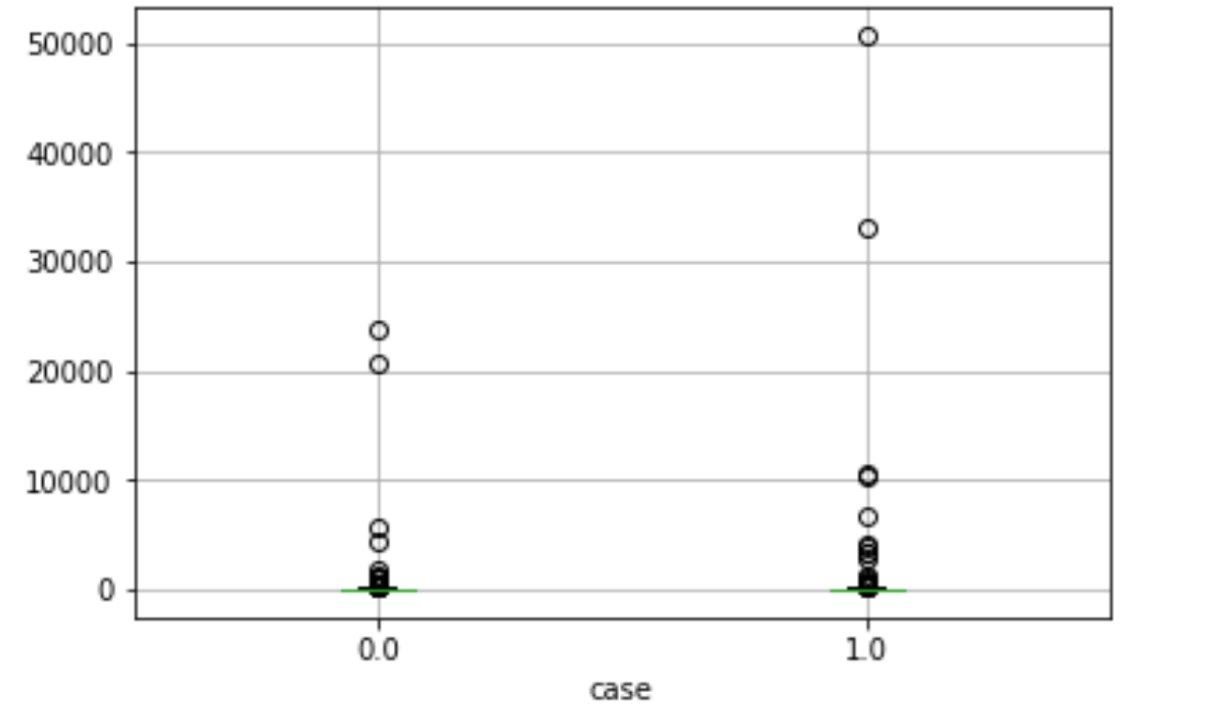
\includegraphics[width=0.5\textwidth,height=\textheight]{source/figures/fibre2.png}
\caption{Boxplot of fibre-ml.year asbestos exposure estimates for cases
and controls for those reporting exposure (N=108)}
\end{figure}

818(85\%) of the 960 participants were genotyped for MUC5b rs3570950.
Being heterozygous for the disease associated variant (GT) had an odds
ratio of 5 (95\%CI 3.7-6.8; p \textless{} 0.001) for disease. Being
homozygous for the disease associated variant (GG) had an odds ratio of
13.3 (95\%CI 5.1-35, p \textless{} 0.001) for disease. Ever having
smoked was associated with increased risk of disease, odds ratio 1.4
(95\%CI 1-1.8, p \textless{} 0.03). There was a statistically
significant interaction between smoking and having ever been been
exposed to a high or medium asbestos exposure risk job, odds ratio for
interaction 1.9 (95\%CI 1.03-3.36, p \textless{} 0.04). Several
non-significant gene-environment interactions were present (see Table
seven).

\hypertarget{table-seven-muc5b-rs35705950-occupational-asbestos-exposure-smoking-and-ipf-risk}{%
\subsubsection{Table seven: MUC5b rs35705950, occupational asbestos
exposure, smoking, and IPF
risk}\label{table-seven-muc5b-rs35705950-occupational-asbestos-exposure-smoking-and-ipf-risk}}

\begin{longtable}[]{@{}ll@{}}
\toprule
Exposure & OR (95\%CI; p-value)\textsuperscript{1}
\textsuperscript{2}\tabularnewline
\midrule
\endhead
rs35705950 &\tabularnewline
GG & 1\tabularnewline
GT & 5 (3.7-6.8; \textless{} 0.001)\tabularnewline
TT & 13.3 (5.1-35; \textless{} 0.001)\tabularnewline
&\tabularnewline
Ever smoked & 1.4 (1-1.8; 0.03)\textsuperscript{3}\tabularnewline
EE interaction (smoking and ever exposed) & 1.9 (1.03-3.36;
0.04)\textsuperscript{3}\tabularnewline
&\tabularnewline
GE interaction (ever exposed) & 1.5 (0.8-2.7; 0.2)\tabularnewline
GE interaction (categories of exposure) & 1.1(0.9-1.4;
0.38)\tabularnewline
GE interaction (fibre-ml years) & 1(0.99-1; 0.34)\tabularnewline
GE interaction (ever smoked) & 1.2 (0.6-2.2; 0.7)\tabularnewline
\bottomrule
\end{longtable}

\textsuperscript{1} additive model, adjusted for age and smoking, N=818
for analysis involving genotype and N=960 for analysis not involving
genotype\\
\textsuperscript{2} adjusted for age only where smoking is exposure\\
\textsuperscript{3} when adjusting for centre also ever smoked remains
significant but smoking and ever exposed does not

The regression coefficient for MUC5b rs35705950 genotype, using an
additive model, was significant but age, smoking, asbestos exposure, and
the interaction of asbestos exposure and genotype were not. See
dot-and-whisker plot of regression coefficients (Figure 6.4).

\begin{figure}
\centering
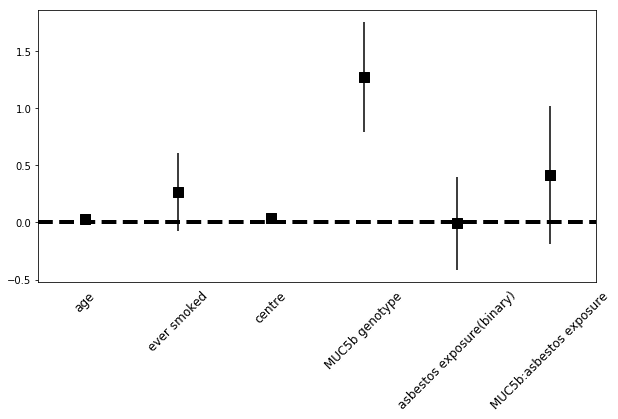
\includegraphics{source/figures/regression_coefficients.png}
\caption{Regression coefficients for logistic regression of case status
against age in years, ever having smoked (binary), centre, MUC5b
rs35705950 genotype (additive model), asbestos exposure (ever held high
or medium risk asbestos exposure job based on job title), and
gene-environment interaction (N=818)}
\end{figure}

Ever having a job with wood, metal, or stone exposure was associated
with disease, odds ratio 1.7 (95\%CI 1.2-2.3, p \textless{} 0.01). Stone
dust exposure alone was associated with a statistically significant odds
ratio for disease of 2.9 (95\%CI 1.3-6.7, p \textless{} 0.01) but wood
and metal dust were not (see Table eight).

\hypertarget{table-eight-occupational-metal-wood-and-stone-exposure-and-ipf-risk}{%
\subsubsection{Table eight: Occupational metal, wood, and stone exposure
and IPF
risk}\label{table-eight-occupational-metal-wood-and-stone-exposure-and-ipf-risk}}

\begin{longtable}[]{@{}lllll@{}}
\toprule
\begin{minipage}[b]{0.20\columnwidth}\raggedright
Exposure\strut
\end{minipage} & \begin{minipage}[b]{0.08\columnwidth}\raggedright
Cases (\%)\strut
\end{minipage} & \begin{minipage}[b]{0.10\columnwidth}\raggedright
Controls (\%)\strut
\end{minipage} & \begin{minipage}[b]{0.24\columnwidth}\raggedright
Unadjusted OR (95\%CI; p-value)\strut
\end{minipage} & \begin{minipage}[b]{0.24\columnwidth}\raggedright
Adjusted OR\textsuperscript{1} (95\%CI; p-value)\strut
\end{minipage}\tabularnewline
\midrule
\endhead
\begin{minipage}[t]{0.20\columnwidth}\raggedright
Wood, metal, stone (any)\strut
\end{minipage} & \begin{minipage}[t]{0.08\columnwidth}\raggedright
139(28)\strut
\end{minipage} & \begin{minipage}[t]{0.10\columnwidth}\raggedright
84(18)\strut
\end{minipage} & \begin{minipage}[t]{0.24\columnwidth}\raggedright
1.8(1.3-2.4; \textless0.01)\strut
\end{minipage} & \begin{minipage}[t]{0.24\columnwidth}\raggedright
1.7(1.2-2.3; \textless0.01)\strut
\end{minipage}\tabularnewline
\begin{minipage}[t]{0.20\columnwidth}\raggedright
Wood\strut
\end{minipage} & \begin{minipage}[t]{0.08\columnwidth}\raggedright
48(10)\strut
\end{minipage} & \begin{minipage}[t]{0.10\columnwidth}\raggedright
31(7)\strut
\end{minipage} & \begin{minipage}[t]{0.24\columnwidth}\raggedright
1.5(0.9-2.4; 0.09)\strut
\end{minipage} & \begin{minipage}[t]{0.24\columnwidth}\raggedright
1.4(0.9-2.3; 0.2)\strut
\end{minipage}\tabularnewline
\begin{minipage}[t]{0.20\columnwidth}\raggedright
Metal\strut
\end{minipage} & \begin{minipage}[t]{0.08\columnwidth}\raggedright
88(18)\strut
\end{minipage} & \begin{minipage}[t]{0.10\columnwidth}\raggedright
57(12)\strut
\end{minipage} & \begin{minipage}[t]{0.24\columnwidth}\raggedright
1.6(1.1-2.2; 0.02)\strut
\end{minipage} & \begin{minipage}[t]{0.24\columnwidth}\raggedright
1.4(0.9-2.0; 0.1)\strut
\end{minipage}\tabularnewline
\begin{minipage}[t]{0.20\columnwidth}\raggedright
Stone\strut
\end{minipage} & \begin{minipage}[t]{0.08\columnwidth}\raggedright
24(5)\strut
\end{minipage} & \begin{minipage}[t]{0.10\columnwidth}\raggedright
8(2)\strut
\end{minipage} & \begin{minipage}[t]{0.24\columnwidth}\raggedright
2.9(1.3-6.6; 0.01)\strut
\end{minipage} & \begin{minipage}[t]{0.24\columnwidth}\raggedright
2.9(1.3-6.7; 0.01)\strut
\end{minipage}\tabularnewline
\bottomrule
\end{longtable}

\textsuperscript{1} Adjusted for age, smoking, and centre

As a result of increasing awareness, and regulation, occupational
asbestos exposure prior to 1980 was significantly more
widespread.{[}@Gilham2018{]} To investigate whether occupational
asbestos exposure might be associated with IPF during this period I
performed a sensitivity analysis by only including participants jobs
that ended before 1980. I did not observe a significant association
(Table nine and ten). I also performed sensitivity analyses limiting to
jobs that started before 1980, participants born prior to 65, and
considering only jobs before age 45{[}@Darnton2012{]}; there was no
significant association between asbestos exposure and IPF for these.

\hypertarget{table-nine-sensitivity-analysis-limited-to-jobs-that-ended-before-1980-occupational-asbestos-exposure-inferred-by-job-title-and-ipf-risk-ever-vs-never}{%
\subsubsection{Table nine: Sensitivity analysis (limited to jobs that
ended before 1980): Occupational asbestos exposure (inferred by job
title) and IPF risk (ever vs
never)}\label{table-nine-sensitivity-analysis-limited-to-jobs-that-ended-before-1980-occupational-asbestos-exposure-inferred-by-job-title-and-ipf-risk-ever-vs-never}}

\begin{longtable}[]{@{}lllll@{}}
\toprule
\begin{minipage}[b]{0.06\columnwidth}\raggedright
\strut
\end{minipage} & \begin{minipage}[b]{0.10\columnwidth}\raggedright
Cases (\%)\strut
\end{minipage} & \begin{minipage}[b]{0.12\columnwidth}\raggedright
Controls (\%)\strut
\end{minipage} & \begin{minipage}[b]{0.29\columnwidth}\raggedright
Unadjusted OR (95\%CI; p-value)\strut
\end{minipage} & \begin{minipage}[b]{0.28\columnwidth}\raggedright
Adjusted OR\textsuperscript{1} (95\%CI; p-value)\strut
\end{minipage}\tabularnewline
\midrule
\endhead
\begin{minipage}[t]{0.06\columnwidth}\raggedright
ever\strut
\end{minipage} & \begin{minipage}[t]{0.10\columnwidth}\raggedright
250(62)\strut
\end{minipage} & \begin{minipage}[t]{0.12\columnwidth}\raggedright
220(59)\strut
\end{minipage} & \begin{minipage}[t]{0.29\columnwidth}\raggedright
1.11(0.8-1.5; 0.46)\strut
\end{minipage} & \begin{minipage}[t]{0.28\columnwidth}\raggedright
0.97(0.72-1.32; 0.87)\strut
\end{minipage}\tabularnewline
\begin{minipage}[t]{0.06\columnwidth}\raggedright
never\strut
\end{minipage} & \begin{minipage}[t]{0.10\columnwidth}\raggedright
156(38)\strut
\end{minipage} & \begin{minipage}[t]{0.12\columnwidth}\raggedright
153(41)\strut
\end{minipage} & \begin{minipage}[t]{0.29\columnwidth}\raggedright
1\strut
\end{minipage} & \begin{minipage}[t]{0.28\columnwidth}\raggedright
1\strut
\end{minipage}\tabularnewline
\bottomrule
\end{longtable}

\textsuperscript{1} Adjusted for age, smoking, and centre

\hypertarget{table-ten-sensitivity-analysis-limited-to-jobs-that-ended-before-1980-occupational-asbestos-exposure-inferred-by-job-title-and-ipf-risk-categories-of-exposure}{%
\subsubsection{Table ten: Sensitivity analysis (limited to jobs that
ended before 1980): Occupational asbestos exposure (inferred by job
title) and IPF risk (categories of
exposure)}\label{table-ten-sensitivity-analysis-limited-to-jobs-that-ended-before-1980-occupational-asbestos-exposure-inferred-by-job-title-and-ipf-risk-categories-of-exposure}}

\begin{longtable}[]{@{}lllll@{}}
\toprule
\begin{minipage}[b]{0.20\columnwidth}\raggedright
Category\strut
\end{minipage} & \begin{minipage}[b]{0.08\columnwidth}\raggedright
Cases (\%)\strut
\end{minipage} & \begin{minipage}[b]{0.10\columnwidth}\raggedright
Controls (\%)\strut
\end{minipage} & \begin{minipage}[b]{0.24\columnwidth}\raggedright
Unadjusted OR (95\%CI; p-value)\strut
\end{minipage} & \begin{minipage}[b]{0.23\columnwidth}\raggedright
Adjusted OR\textsuperscript{1} (95\%CI; p-value)\strut
\end{minipage}\tabularnewline
\midrule
\endhead
\begin{minipage}[t]{0.20\columnwidth}\raggedright
high-risk non-construction\strut
\end{minipage} & \begin{minipage}[t]{0.08\columnwidth}\raggedright
53(13)\strut
\end{minipage} & \begin{minipage}[t]{0.10\columnwidth}\raggedright
36(10)\strut
\end{minipage} & \begin{minipage}[t]{0.24\columnwidth}\raggedright
1.55(0.9-2.6;0.62)\strut
\end{minipage} & \begin{minipage}[t]{0.23\columnwidth}\raggedright
1.09(0.61-1.94;0.77)\strut
\end{minipage}\tabularnewline
\begin{minipage}[t]{0.20\columnwidth}\raggedright
high-risk construction\strut
\end{minipage} & \begin{minipage}[t]{0.08\columnwidth}\raggedright
95(23)\strut
\end{minipage} & \begin{minipage}[t]{0.10\columnwidth}\raggedright
81(22)\strut
\end{minipage} & \begin{minipage}[t]{0.24\columnwidth}\raggedright
1.22(0.8-1.9;0.88)\strut
\end{minipage} & \begin{minipage}[t]{0.23\columnwidth}\raggedright
1.01(0.63-1.63;0.97)\strut
\end{minipage}\tabularnewline
\begin{minipage}[t]{0.20\columnwidth}\raggedright
medium risk industrial\strut
\end{minipage} & \begin{minipage}[t]{0.08\columnwidth}\raggedright
102(25)\strut
\end{minipage} & \begin{minipage}[t]{0.10\columnwidth}\raggedright
103(28)\strut
\end{minipage} & \begin{minipage}[t]{0.24\columnwidth}\raggedright
1.03(0.7-1.6;0.37)\strut
\end{minipage} & \begin{minipage}[t]{0.23\columnwidth}\raggedright
0.83(0.52-1.33;0.44)\strut
\end{minipage}\tabularnewline
\begin{minipage}[t]{0.20\columnwidth}\raggedright
low risk industrial\strut
\end{minipage} & \begin{minipage}[t]{0.08\columnwidth}\raggedright
90(22)\strut
\end{minipage} & \begin{minipage}[t]{0.10\columnwidth}\raggedright
84(23)\strut
\end{minipage} & \begin{minipage}[t]{0.24\columnwidth}\raggedright
1.12(0.7-1.8;0.12)\strut
\end{minipage} & \begin{minipage}[t]{0.23\columnwidth}\raggedright
0.94(0.58-1.52;0.8)\strut
\end{minipage}\tabularnewline
\begin{minipage}[t]{0.20\columnwidth}\raggedright
office\strut
\end{minipage} & \begin{minipage}[t]{0.08\columnwidth}\raggedright
66(16)\strut
\end{minipage} & \begin{minipage}[t]{0.10\columnwidth}\raggedright
69(18)\strut
\end{minipage} & \begin{minipage}[t]{0.24\columnwidth}\raggedright
1\strut
\end{minipage} & \begin{minipage}[t]{0.23\columnwidth}\raggedright
1\strut
\end{minipage}\tabularnewline
\bottomrule
\end{longtable}

\textsuperscript{1} Adjusted for age, smoking, and centre

I considered that a minimum duration in a high or medium risk job might
be important and performed a sensitivity analysis limited to jobs of
five or more years in duration (See table eleven and twelve and figure
6.5)

\newpage

\hypertarget{table-eleven-sensitivity-analysis-limited-to-jobs-that-spent-minimum-of-5-years-in-occupational-asbestos-exposure-inferred-by-job-title-and-ipf-risk-ever-vs-never}{%
\subsubsection{Table eleven: Sensitivity analysis (limited to jobs that
spent minimum of 5 years in): Occupational asbestos exposure (inferred
by job title) and IPF risk (ever vs
never)}\label{table-eleven-sensitivity-analysis-limited-to-jobs-that-spent-minimum-of-5-years-in-occupational-asbestos-exposure-inferred-by-job-title-and-ipf-risk-ever-vs-never}}

\begin{longtable}[]{@{}lllll@{}}
\toprule
\begin{minipage}[b]{0.06\columnwidth}\raggedright
\strut
\end{minipage} & \begin{minipage}[b]{0.10\columnwidth}\raggedright
Cases (\%)\strut
\end{minipage} & \begin{minipage}[b]{0.12\columnwidth}\raggedright
Controls (\%)\strut
\end{minipage} & \begin{minipage}[b]{0.29\columnwidth}\raggedright
Unadjusted OR (95\%CI; p-value)\strut
\end{minipage} & \begin{minipage}[b]{0.28\columnwidth}\raggedright
Adjusted OR\textsuperscript{1} (95\%CI; p-value)\strut
\end{minipage}\tabularnewline
\midrule
\endhead
\begin{minipage}[t]{0.06\columnwidth}\raggedright
ever\strut
\end{minipage} & \begin{minipage}[t]{0.10\columnwidth}\raggedright
257(52)\strut
\end{minipage} & \begin{minipage}[t]{0.12\columnwidth}\raggedright
235(51)\strut
\end{minipage} & \begin{minipage}[t]{0.29\columnwidth}\raggedright
1.06(0.82-1.37; 0.65)\strut
\end{minipage} & \begin{minipage}[t]{0.28\columnwidth}\raggedright
0.93(0.71-1.22; 0.63)\strut
\end{minipage}\tabularnewline
\begin{minipage}[t]{0.06\columnwidth}\raggedright
never\strut
\end{minipage} & \begin{minipage}[t]{0.10\columnwidth}\raggedright
237(48)\strut
\end{minipage} & \begin{minipage}[t]{0.12\columnwidth}\raggedright
230(49)\strut
\end{minipage} & \begin{minipage}[t]{0.29\columnwidth}\raggedright
1\strut
\end{minipage} & \begin{minipage}[t]{0.28\columnwidth}\raggedright
1\strut
\end{minipage}\tabularnewline
\bottomrule
\end{longtable}

\textsuperscript{1} Adjusted for age, smoking, and centre

\hypertarget{table-twelve-sensitivity-analysis-limited-to-jobs-that-spent-minimum-of-5-years-in-occupational-asbestos-exposure-inferred-by-job-title-and-ipf-risk-categories-of-exposure}{%
\subsubsection{Table twelve: Sensitivity analysis (limited to jobs that
spent minimum of 5 years in): Occupational asbestos exposure (inferred
by job title) and IPF risk (categories of
exposure)}\label{table-twelve-sensitivity-analysis-limited-to-jobs-that-spent-minimum-of-5-years-in-occupational-asbestos-exposure-inferred-by-job-title-and-ipf-risk-categories-of-exposure}}

\begin{longtable}[]{@{}lllll@{}}
\toprule
\begin{minipage}[b]{0.20\columnwidth}\raggedright
Category\strut
\end{minipage} & \begin{minipage}[b]{0.08\columnwidth}\raggedright
Cases (\%)\strut
\end{minipage} & \begin{minipage}[b]{0.10\columnwidth}\raggedright
Controls (\%)\strut
\end{minipage} & \begin{minipage}[b]{0.24\columnwidth}\raggedright
Unadjusted OR (95\%CI; p-value)\strut
\end{minipage} & \begin{minipage}[b]{0.23\columnwidth}\raggedright
Adjusted OR\textsuperscript{1} (95\%CI; p-value)\strut
\end{minipage}\tabularnewline
\midrule
\endhead
\begin{minipage}[t]{0.20\columnwidth}\raggedright
high-risk non-construction\strut
\end{minipage} & \begin{minipage}[t]{0.08\columnwidth}\raggedright
34(7)\strut
\end{minipage} & \begin{minipage}[t]{0.10\columnwidth}\raggedright
32(7)\strut
\end{minipage} & \begin{minipage}[t]{0.24\columnwidth}\raggedright
0.93(0.55-1.6;0.47)\strut
\end{minipage} & \begin{minipage}[t]{0.23\columnwidth}\raggedright
0.68(0.38-1.22;0.2)\strut
\end{minipage}\tabularnewline
\begin{minipage}[t]{0.20\columnwidth}\raggedright
high-risk construction\strut
\end{minipage} & \begin{minipage}[t]{0.08\columnwidth}\raggedright
115(23)\strut
\end{minipage} & \begin{minipage}[t]{0.10\columnwidth}\raggedright
98(22)\strut
\end{minipage} & \begin{minipage}[t]{0.24\columnwidth}\raggedright
1.03(0.71-1.5;0.39)\strut
\end{minipage} & \begin{minipage}[t]{0.23\columnwidth}\raggedright
0.94(0.64-1.4;0.78)\strut
\end{minipage}\tabularnewline
\begin{minipage}[t]{0.20\columnwidth}\raggedright
medium risk industrial\strut
\end{minipage} & \begin{minipage}[t]{0.08\columnwidth}\raggedright
108(22)\strut
\end{minipage} & \begin{minipage}[t]{0.10\columnwidth}\raggedright
105(23)\strut
\end{minipage} & \begin{minipage}[t]{0.24\columnwidth}\raggedright
0.9(0.63-1.3;0.26)\strut
\end{minipage} & \begin{minipage}[t]{0.23\columnwidth}\raggedright
0.72(0.49-1.07;0.11)\strut
\end{minipage}\tabularnewline
\begin{minipage}[t]{0.20\columnwidth}\raggedright
low risk industrial\strut
\end{minipage} & \begin{minipage}[t]{0.08\columnwidth}\raggedright
99(20)\strut
\end{minipage} & \begin{minipage}[t]{0.10\columnwidth}\raggedright
109(23)\strut
\end{minipage} & \begin{minipage}[t]{0.24\columnwidth}\raggedright
0.79(0.55-1.48;0.14)\strut
\end{minipage} & \begin{minipage}[t]{0.23\columnwidth}\raggedright
0.73(0.49-1.08;0.34)\strut
\end{minipage}\tabularnewline
\begin{minipage}[t]{0.20\columnwidth}\raggedright
office\strut
\end{minipage} & \begin{minipage}[t]{0.08\columnwidth}\raggedright
138(28)\strut
\end{minipage} & \begin{minipage}[t]{0.10\columnwidth}\raggedright
121(26)\strut
\end{minipage} & \begin{minipage}[t]{0.24\columnwidth}\raggedright
1\strut
\end{minipage} & \begin{minipage}[t]{0.23\columnwidth}\raggedright
1\strut
\end{minipage}\tabularnewline
\bottomrule
\end{longtable}

\textsuperscript{1} Adjusted for age, smoking, and centre

\begin{figure}
\centering
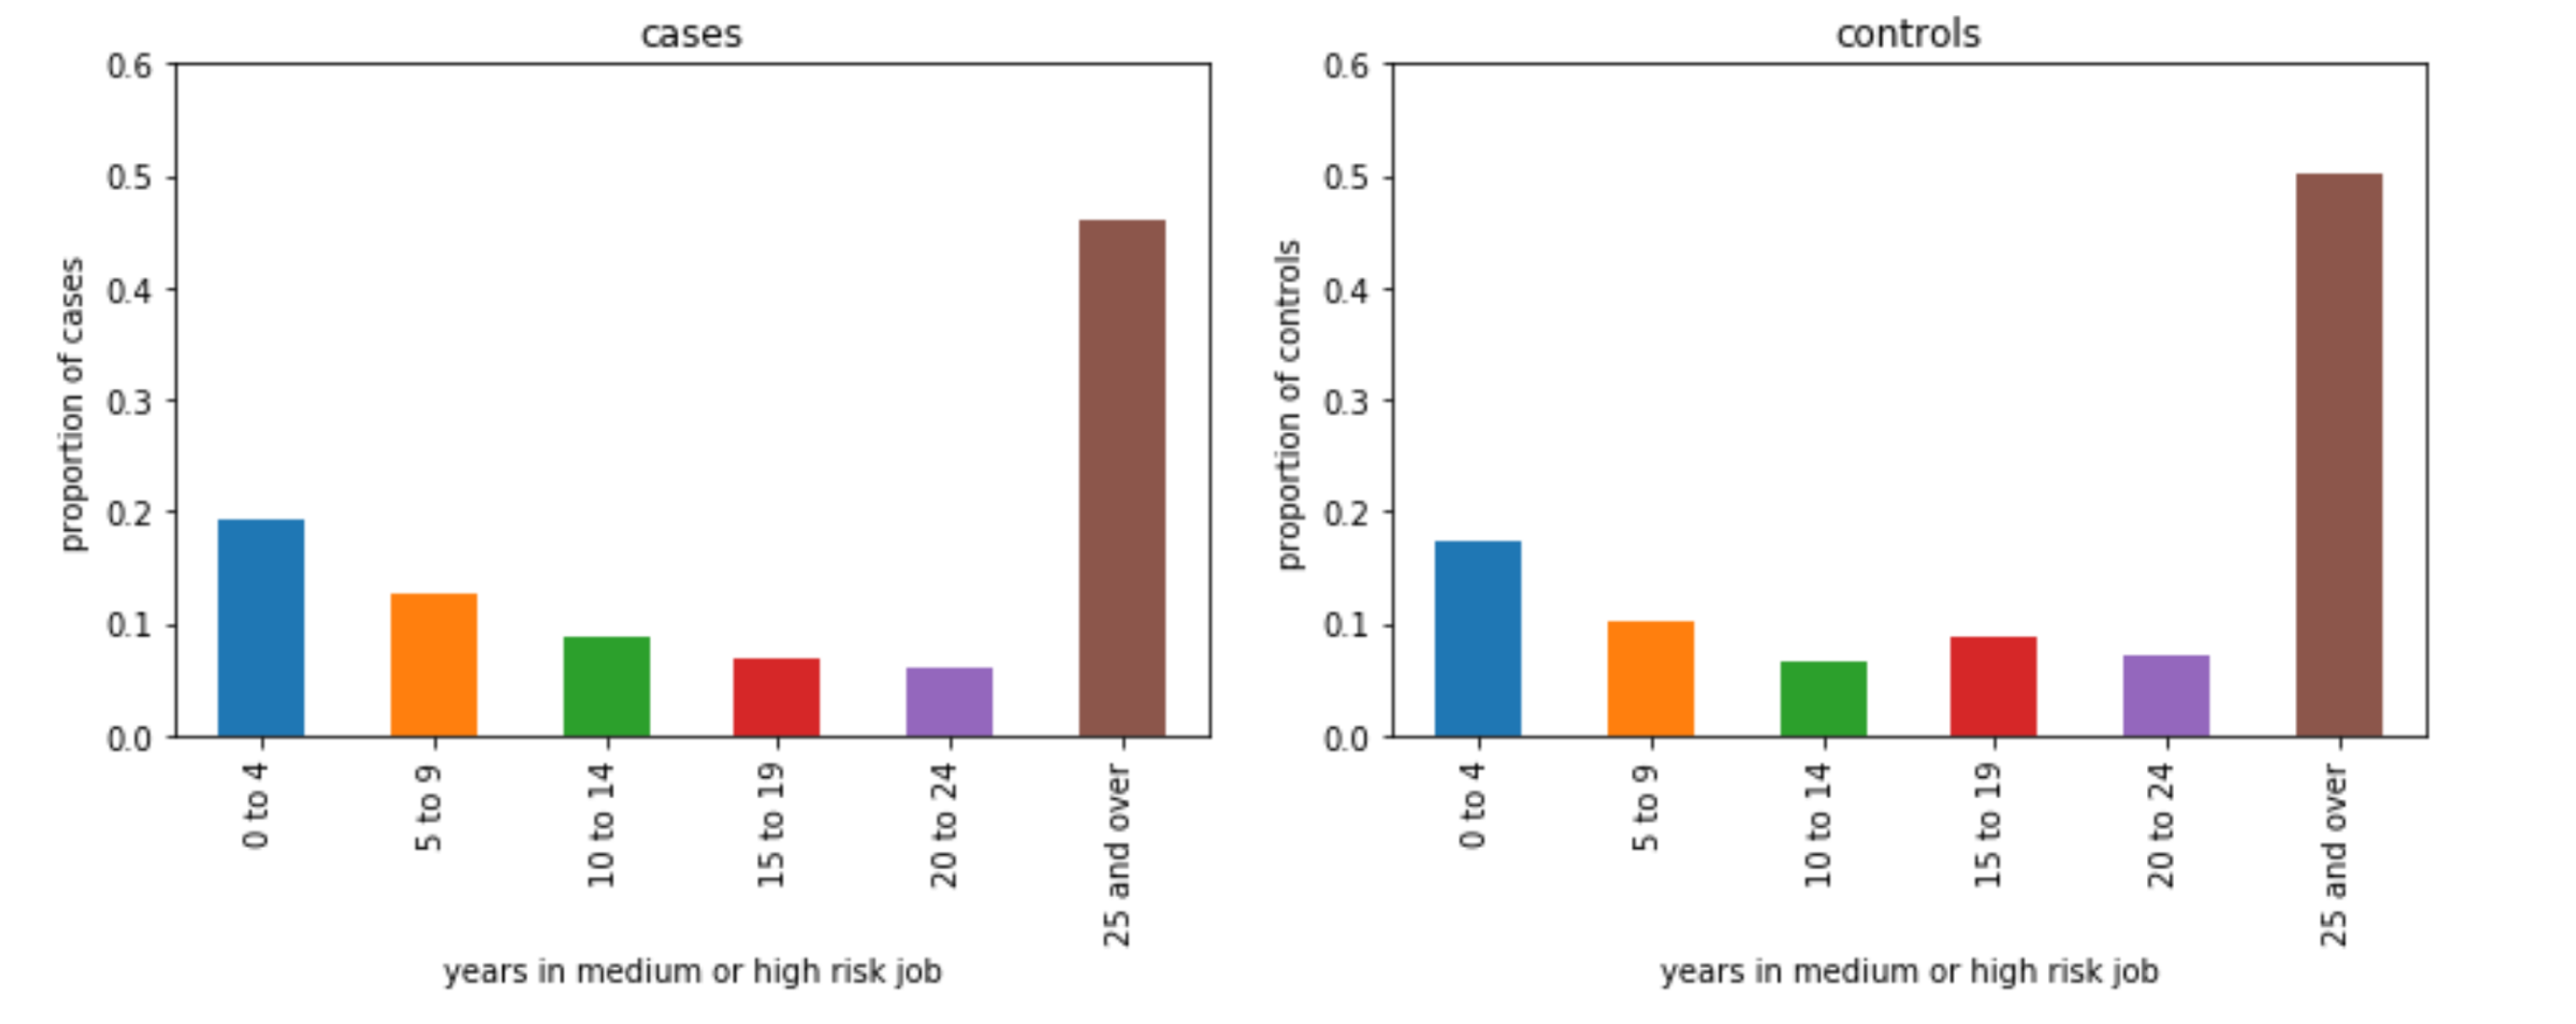
\includegraphics{source/figures/years.png}
\caption{Years in a medium or high risk asbestos exposure job for cases
and controls (N=492)}
\end{figure}

Cases and controls lived an average of 28km and 16km respectively from
their recruiting hospital, measured by calculating the distance between
the postcode centroid of the participants general practice and the
postcode centroid of the hospital. Living further away from the hospital
correlated with being a case, r=0.22, 95\%CI = 0.16-0.29, p \textless{}
0.001 and weakly correlated with reduced asbestos exposure, r=-0.06,
95\%CI = -0.13-0, p=0.05. To investigate this further I performed a
sensitivity analysis limited to participants within 10km of their
recruiting hospital (Table thirteen and fourteen).

\hypertarget{table-thirteen-sensitivity-analysis-limited-to-participants-within-10km-of-the-hospital-occupational-asbestos-exposure-inferred-by-job-title-and-ipf-risk-ever-vs-never}{%
\subsubsection{Table thirteen: Sensitivity analysis (limited to
participants within 10km of the hospital): Occupational asbestos
exposure (inferred by job title) and IPF risk (ever vs
never)}\label{table-thirteen-sensitivity-analysis-limited-to-participants-within-10km-of-the-hospital-occupational-asbestos-exposure-inferred-by-job-title-and-ipf-risk-ever-vs-never}}

\begin{longtable}[]{@{}lllll@{}}
\toprule
\begin{minipage}[b]{0.06\columnwidth}\raggedright
\strut
\end{minipage} & \begin{minipage}[b]{0.10\columnwidth}\raggedright
Cases (\%)\strut
\end{minipage} & \begin{minipage}[b]{0.12\columnwidth}\raggedright
Controls (\%)\strut
\end{minipage} & \begin{minipage}[b]{0.29\columnwidth}\raggedright
Unadjusted OR (95\%CI; p-value)\strut
\end{minipage} & \begin{minipage}[b]{0.28\columnwidth}\raggedright
Adjusted OR\textsuperscript{1} (95\%CI; p-value)\strut
\end{minipage}\tabularnewline
\midrule
\endhead
\begin{minipage}[t]{0.06\columnwidth}\raggedright
ever\strut
\end{minipage} & \begin{minipage}[t]{0.10\columnwidth}\raggedright
111(73)\strut
\end{minipage} & \begin{minipage}[t]{0.12\columnwidth}\raggedright
180(64)\strut
\end{minipage} & \begin{minipage}[t]{0.29\columnwidth}\raggedright
1.46(0.95-2.26; 0.08)\strut
\end{minipage} & \begin{minipage}[t]{0.28\columnwidth}\raggedright
1.33(0.82-2.16; 0.24)\strut
\end{minipage}\tabularnewline
\begin{minipage}[t]{0.06\columnwidth}\raggedright
never\strut
\end{minipage} & \begin{minipage}[t]{0.10\columnwidth}\raggedright
42(27)\strut
\end{minipage} & \begin{minipage}[t]{0.12\columnwidth}\raggedright
100(36)\strut
\end{minipage} & \begin{minipage}[t]{0.29\columnwidth}\raggedright
1\strut
\end{minipage} & \begin{minipage}[t]{0.28\columnwidth}\raggedright
1\strut
\end{minipage}\tabularnewline
\bottomrule
\end{longtable}

\textsuperscript{1} Adjusted for age, smoking, and centre

\hypertarget{table-fourteen-sensitivity-analysis-limited-to-participants-within-10km-of-the-hospital-occupational-asbestos-exposure-inferred-by-job-title-and-ipf-risk-categories-of-exposure}{%
\subsubsection{Table fourteen: Sensitivity analysis (limited to
participants within 10km of the hospital): Occupational asbestos
exposure (inferred by job title) and IPF risk (categories of
exposure)}\label{table-fourteen-sensitivity-analysis-limited-to-participants-within-10km-of-the-hospital-occupational-asbestos-exposure-inferred-by-job-title-and-ipf-risk-categories-of-exposure}}

\begin{longtable}[]{@{}lllll@{}}
\toprule
\begin{minipage}[b]{0.20\columnwidth}\raggedright
Category\strut
\end{minipage} & \begin{minipage}[b]{0.08\columnwidth}\raggedright
Cases (\%)\strut
\end{minipage} & \begin{minipage}[b]{0.10\columnwidth}\raggedright
Controls (\%)\strut
\end{minipage} & \begin{minipage}[b]{0.24\columnwidth}\raggedright
Unadjusted OR (95\%CI; p-value)\strut
\end{minipage} & \begin{minipage}[b]{0.23\columnwidth}\raggedright
Adjusted OR\textsuperscript{1} (95\%CI; p-value)\strut
\end{minipage}\tabularnewline
\midrule
\endhead
\begin{minipage}[t]{0.20\columnwidth}\raggedright
high-risk non-construction\strut
\end{minipage} & \begin{minipage}[t]{0.08\columnwidth}\raggedright
23(15)\strut
\end{minipage} & \begin{minipage}[t]{0.10\columnwidth}\raggedright
35(13)\strut
\end{minipage} & \begin{minipage}[t]{0.24\columnwidth}\raggedright
1.62(0.75-3.51;0.22)\strut
\end{minipage} & \begin{minipage}[t]{0.23\columnwidth}\raggedright
1.05(0.44-2.52;0.9)\strut
\end{minipage}\tabularnewline
\begin{minipage}[t]{0.20\columnwidth}\raggedright
high-risk construction\strut
\end{minipage} & \begin{minipage}[t]{0.08\columnwidth}\raggedright
47(31)\strut
\end{minipage} & \begin{minipage}[t]{0.10\columnwidth}\raggedright
80(29)\strut
\end{minipage} & \begin{minipage}[t]{0.24\columnwidth}\raggedright
1.45(0.74-2.83;0.23)\strut
\end{minipage} & \begin{minipage}[t]{0.23\columnwidth}\raggedright
1.21(0.58-2.52;0.62)\strut
\end{minipage}\tabularnewline
\begin{minipage}[t]{0.20\columnwidth}\raggedright
medium risk industrial\strut
\end{minipage} & \begin{minipage}[t]{0.08\columnwidth}\raggedright
41(27)\strut
\end{minipage} & \begin{minipage}[t]{0.10\columnwidth}\raggedright
65(23)\strut
\end{minipage} & \begin{minipage}[t]{0.24\columnwidth}\raggedright
1.55(0.78-3.09;0.21)\strut
\end{minipage} & \begin{minipage}[t]{0.23\columnwidth}\raggedright
0.93(0.43-2.04;0.86)\strut
\end{minipage}\tabularnewline
\begin{minipage}[t]{0.20\columnwidth}\raggedright
low risk industrial\strut
\end{minipage} & \begin{minipage}[t]{0.08\columnwidth}\raggedright
25(16)\strut
\end{minipage} & \begin{minipage}[t]{0.10\columnwidth}\raggedright
58(21)\strut
\end{minipage} & \begin{minipage}[t]{0.24\columnwidth}\raggedright
1.06(0.51-2.21;0.87)\strut
\end{minipage} & \begin{minipage}[t]{0.23\columnwidth}\raggedright
0.69(0.31-1.59;0.39)\strut
\end{minipage}\tabularnewline
\begin{minipage}[t]{0.20\columnwidth}\raggedright
office\strut
\end{minipage} & \begin{minipage}[t]{0.08\columnwidth}\raggedright
17(11)\strut
\end{minipage} & \begin{minipage}[t]{0.10\columnwidth}\raggedright
42(15)\strut
\end{minipage} & \begin{minipage}[t]{0.24\columnwidth}\raggedright
1\strut
\end{minipage} & \begin{minipage}[t]{0.23\columnwidth}\raggedright
1\strut
\end{minipage}\tabularnewline
\bottomrule
\end{longtable}

\textsuperscript{1} Adjusted for age, smoking, and centre

To investigate cumulative `dose' of exposure based on job title a score
was assigned based on asbestos exposure risk category of each job as
follows:

\begin{itemize}
\tightlist
\item
  high-risk non-construction : 2
\item
  high-risk construction : 2
\item
  medium risk industrial : 1
\item
  low risk industrial : 0
\item
  office : 0
\end{itemize}

Scores were then multiplied for each job by the duration in years of the
job and then summed at participant level. See Table fifteen and Figure
6.6.

\hypertarget{table-fifteen-sensitivity-analyses-cumulative-dose-based-on-occupational-asbestos-exposure-inferred-by-job-title}{%
\subsubsection{Table fifteen: Sensitivity analyses: cumulative `dose'
based on occupational asbestos exposure (inferred by job
title)}\label{table-fifteen-sensitivity-analyses-cumulative-dose-based-on-occupational-asbestos-exposure-inferred-by-job-title}}

\begin{longtable}[]{@{}lllllllll@{}}
\toprule
& N & mean & std & min & 25\% & 50\% & 75\% & max\tabularnewline
\midrule
\endhead
cases & 494 & 23.9 & 30.8 & 0 & 0 & 9 & 40 & 126\tabularnewline
controls & 466 & 24 & 30.4 & 0 & 0 & 6.5 & 42 & 118\tabularnewline
\bottomrule
\end{longtable}

\begin{figure}
\centering
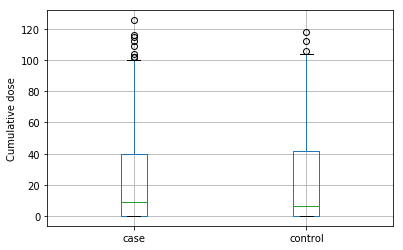
\includegraphics[width=0.5\textwidth,height=\textheight]{source/figures/dose.png}
\caption{Boxplot of cumulative asbestos exposure estimates (inferred
from job title) for cases and controls (N=960)}
\end{figure}

310 (63\%) of IPF cases initially presented to their doctor with cough
and 306 (62\%) with breathlessness (91 patients presented with cough and
breathlessness). 15 (3\%) of cases and 42 (9\%) of controls reported
ever taking a medication suspected of causing usual interstitial
pneumonia (amiodarone, azathioprine, bleomycin, flecainide, gefitinib,
ifosamide, melphalan, and nitrofurantoin).{[}@Bonniaud2014{]}

414 (83\%) of cases and 441 (95\%) of controls reported one or more
comorbidities. The most commonly reported comorbidities (occurring in at
least 10 cases or controls) occurred at a similar frequency in cases and
controls and included hypertension, type II diabetes mellitus,
hypercholesterolemia, ischaemic heart disease, atrial fibrillation,
COPD, osteoarthritis, and prostate cancer. Rheumatoid arthritis was
reported in 18 cases, approximately 2\% of cases reporting a
comorbidity, and in 9 controls, approximately 1\% of controls reporting
a comorbidity. Gastro-oesophageal reflux disease (GORD) was reported in
14 cases, approximately 1.5\% of cases reporting a comorbidity, and in 2
controls, approximately 0.5\% of controls reporting a comorbidity.

Dyspnoea, as measured by the mMRC dyspnoea scale was associated with
case-status, smoking status, genotype, and asbestos exposure. Pearson's
correlation coefficient for IPF was 0.49 (95\%CI 0.44-0.53,
p\textless0.001), ever smoking was 0.16 (95\%CI 0.09-0.23,
p\textless0.001), pack-year smoked was 0.2 (95\%CI 0.13-0.26,
p\textless0.001), genotype 0.2 (95\%CI 0.13-0.27, p\textless0.001), ever
held a medium or high risk asbestos exposure job title 0.09 (95\%CI
0.02-0.16, p=0.02), and 0.15 (95\%CI 0.08-0.21, p\textless0.001) for
having a fibre-ml.year estimate \textgreater{} 25. See Table sixteen and
seventeen for ordinal logistic regression results.

\hypertarget{table-sixteen-ordinal-logistic-regression-for-mmrc-score-and-ever-exposed-to-asbestos}{%
\subsubsection{Table sixteen: Ordinal logistic regression for mMRC score
and ever exposed to
asbestos}\label{table-sixteen-ordinal-logistic-regression-for-mmrc-score-and-ever-exposed-to-asbestos}}

\begin{longtable}[]{@{}lll@{}}
\toprule
& Unadjusted OR (95\%CI; p-value) & Adjusted OR\textsuperscript{1}
(95\%CI; p-value)\tabularnewline
\midrule
\endhead
case & 6.94(5.38-9; \textless0.001) & 6.8 (5.25-8.8;
\textless0.001)\tabularnewline
pack-years & 1.01(1-1.02;\textless0.001) & 1.02(1.01-1.02;
\textless0.001)\tabularnewline
ever exposed\textsuperscript{2} & 1.48(1.17-1.87; \textless0.001) &
1.44(1.12-1.84; 0.004)\tabularnewline
\bottomrule
\end{longtable}

\textsuperscript{1} Adjusted for age, smoking (pack-years), and case
status \textsuperscript{2} Ever exposed to a high or medium asbestos
exposure job (inferred from job title)

\hypertarget{table-seventeen-ordinal-logistic-regression-for-mmrc-score-and-for-categories-of-asbestos-exposure}{%
\subsubsection{Table seventeen: Ordinal logistic regression for mMRC
score and for categories of asbestos
exposure}\label{table-seventeen-ordinal-logistic-regression-for-mmrc-score-and-for-categories-of-asbestos-exposure}}

\begin{longtable}[]{@{}lll@{}}
\toprule
Category & Unadjusted OR (95\%CI; p-value) & Adjusted
OR\textsuperscript{1} (95\%CI; p-value)\tabularnewline
\midrule
\endhead
high-risk non-construction & 2.21(1.43-3.44;\textless0.001) &
1.92(1.2-3.03;0.006)\tabularnewline
high-risk construction & 1.9(1.31-2.74;0.001) &
1.89(1.29-2.78;0.001)\tabularnewline
medium risk industrial & 1.36(0.94-1.98;0.103) &
1.28(0.87-1.89;0.21)\tabularnewline
low risk industrial & 1.29(0.88-1.9;0.19) &
1.24(0.82-1.87;0.29)\tabularnewline
office & 1 & 1\tabularnewline
\bottomrule
\end{longtable}

\textsuperscript{1} Adjusted for age, smoking (pack-years), and case
status

\hypertarget{discussion-3}{%
\subsection{Discussion}\label{discussion-3}}

\hypertarget{findings-interpretation-implications-relations-ot-others-work-limitations-strengths}{%
\subsubsection{findings, interpretation, implications, relations ot
others work, limitations,
strengths}\label{findings-interpretation-implications-relations-ot-others-work-limitations-strengths}}

494 cases and 466 controls were recruited and interviewed. The median
age of cases was 76 years and controls 74 years. 97\% of cases and 96\%
of controls reported their ethnicity as white and social economic class
and exposure to smoking were similar for cases and controls (see Table
1). Cases were less likely than controls to have ever been prescribed
medications known to cause UIP, 15(3\%) versus 42(9\%) respectively.
Cases were more likely than controls to be breathless, Pearson's
correlation coefficient for mMRC dyspnoea and case status was 0.49
(95\%CI 0.44-0.53, p\textless0.001), adjusted OR for was 6.8 (95\%CI
5.25-8.8; p\textless0.001). Cases were also more likely to have
gastro-oesophageal reflux disease than controls, 14(2\%) versus
2(0.5\%), a known association.{[}@Raghu2006a{]} After controlling for
case and smoking status being ever exposed to a high or medium asbestos
exposure risk job was associated with dyspnoea, measured using ordinal
logistic regression and mMRC dyspnoea score, OR 1.44(1.12-1.84;
p=0.004). The strength of association between asbestos exposure and
dyspnoea increased with increasing categories of asbestos exposure risk.

Ever being exposed to an occupation with high or medium risk for
asbestos exposure was common for both cases (67\%) and controls (63\%)
and the difference in the proportion ever exposed between cases and
controls was not significant (Table four). A similar pattern was
observed for categories of exposure (Table five). 8\% of cases and
controls had estimated cumulative asbestos fibre-ml.year exposures in
excess of 25 fibre-ml.years, the Helsinki criteria exposure threshold at
which cases of asbestosis may occur.{[}@Wolff2015{]} The majority of
these participants had high or medium risk occupations as defined by job
title with carpenter being the single most common job title accounting
for 5\% of all estimates in excess of 25 fibre-ml.years. We found a
significant association with occupational exposure to stone dust and
IPF, OR 2.9(1.3-6.7; 0.01).

In common with numerous previous studies we found MUC5b rs3570950 to be
strongly associated with disease in a risk allele dose-dependant
fashion. We found no evidence of interaction between asbestos exposure
MUC5b rs3570950. However, we did find a significant association for
having ever smoked, OR 1.4 (95\%CI 1-1.8, p \textless{} 0.03) and for
having ever smoked and having ever had a high or medium asbestos
exposure risk based on job title, OR 1.9 (95\%CI 1.03-3.36, p
\textless{} 0.04). Sensitivity analyses including limiting jobs
considered to only those that ended before 1980, considering only jobs
with a duration greater than 5 years, considering only participants
living within 10km of their recruiting hospital, and considering
cumulative exposure `dose' based on summing years in different asbestos
exposure risk categories (assigned by job title) at participant level,
were all non-significant.

Cases and controls were well matched and there was no significant
association between asbestos exposure, measured by well validated means
by job title or by historic asbestos exposure reconstruction, and IPF.
There are three main possible explanations for this:

\begin{enumerate}
\def\labelenumi{\arabic{enumi}.}
\tightlist
\item
  Asbestos exposure is not an important cause of IPF
\item
  Asbestos exposure is only an important cause in concert with other
  environmental or genetic exposures
\item
  Asbestos exposure has not been measured accurately enough in IPFJES
\end{enumerate}

8\% of cases apparently meet the Helsinki criteria for a diagnosis of
asbestosis.{[}@Wolff2015{]} This criterion has been criticised for
failing to reflect the linear dose-response relationship, and lack of
threshold, observed in the published
literature.{[}@Stayner1997{]}{[}@Hein2007{]}{[}@Baur2016{]} Strictly,
IPF is a diagnosis of exclusion that should not be made until exposures
to asbestos, and other known causes of fibrosis, have been
excluded.{[}@Raghu2011{]}{[}@Baur2016{]} Taken to its logical conclusion
this line of argument may result in no diagnoses of IPF in the UK since
asbestos exposure is ubiquitous; the average asbestos lung burden in men
and women without occupational asbestos exposure was recently measured
at approximately 1 fibre/mg of lung tissue.{[}@Gilham2018{]} In IPFJES
the population attributable fraction (PAF) calculated using the
adjusted, non-significant, odds ratio (OR) for ever exposed and
proportion of cases ever exposed (pc) and the equation:
PAF = pc(OR − 1)/OR{[}@Blanc2019{]} is about 5\%.

Of note asbestosis is not necessarily fatal{[}@Doll1985{]} and may not
even be symptomatic since diagnostic criteria require evidence of
scarring of the lungs and evidence of asbestos exposure but not the
presence of symptoms.{[}@Wolff2015{]} In this context a cut off below
which exposure is unlikely to cause significant morbidity or mortality
seems reasonable. Intriguingly our results support the concept of
asbestos exposure being associated with dyspnoea independent of having
IPF and smoking status.

In epidemiological studies the death rate from asbestosis and prevalence
of signs and symptoms to it are both higher in cigarette smokers than
non-smokers.{[}@Doll1985{]} In mouse studies cigarette smoke and
asbestos exposure increase the production of reactive oxygen species
that are thought to be important in the pathogenesis of
asbestosis.{[}@Liu2013{]} Asbestos fibres activates Nalp3 inflammasomes
and cigarette smoke is thought to attenuate the innate immune response
to asbestos through Nalp3 inflammasome suppression.{[}@Morris2015{]}
This is compatible with our observation of an interaction between
asbestos exposure, as measured by ever having a job at medium or high
risk for asbestos exposure, and ever having smoked on IPF risk, OR 1.9
(95\%CI 1.03-3.36, p=0.04).

There is a precedent for the importance of genetic susceptibility in the
development of disease in response to asbestiform fibre inhalation;
specifically germline BAP1 mutations were discovered to be important
together with eronite exposure in the Cappodecia mesothelioma
epidemic.{[}@Testa2011{]}{[}@Emri2017{]} It is possible that there
unmeasured genetic modifiers of asbestos exposure risk the presence, or
absence, of which is necessary for the development of disease.

Despite best efforts it is still theoretically possible that my asbestos
exposure measure was insufficiently sensitive. Review of all
occupational histories by a trained occupational hygeinist blind to the
case status of participants would have been desirable but was was
prohibitively expensive. It is also possible that the underlying data on
which to base historic assessments is not detailed enough to permit
sufficiently sensitive assessments by any means.

Asbestosis can have a latency of upwards of 40 years{[}@Harding2010{]}
and rates have not yet peaked in the UK.{[}@HSE2019{]} From 1900 until
around 1960 (see Figure 2), when asbestos consumption in the United
Kingdom peaked, the United Kingdom had the third highest per capita
asbestos consumption in the world with only to the United States and
later Australia having higher rates of consumption.{[}@Allen2017{]} Our
results are likely to generalize well globally where, with the exception
of Brasil, Russian, India, Iran, and China which continue to consume
asbestos, consumption has been lower and peaked later.

\begin{figure}
\centering
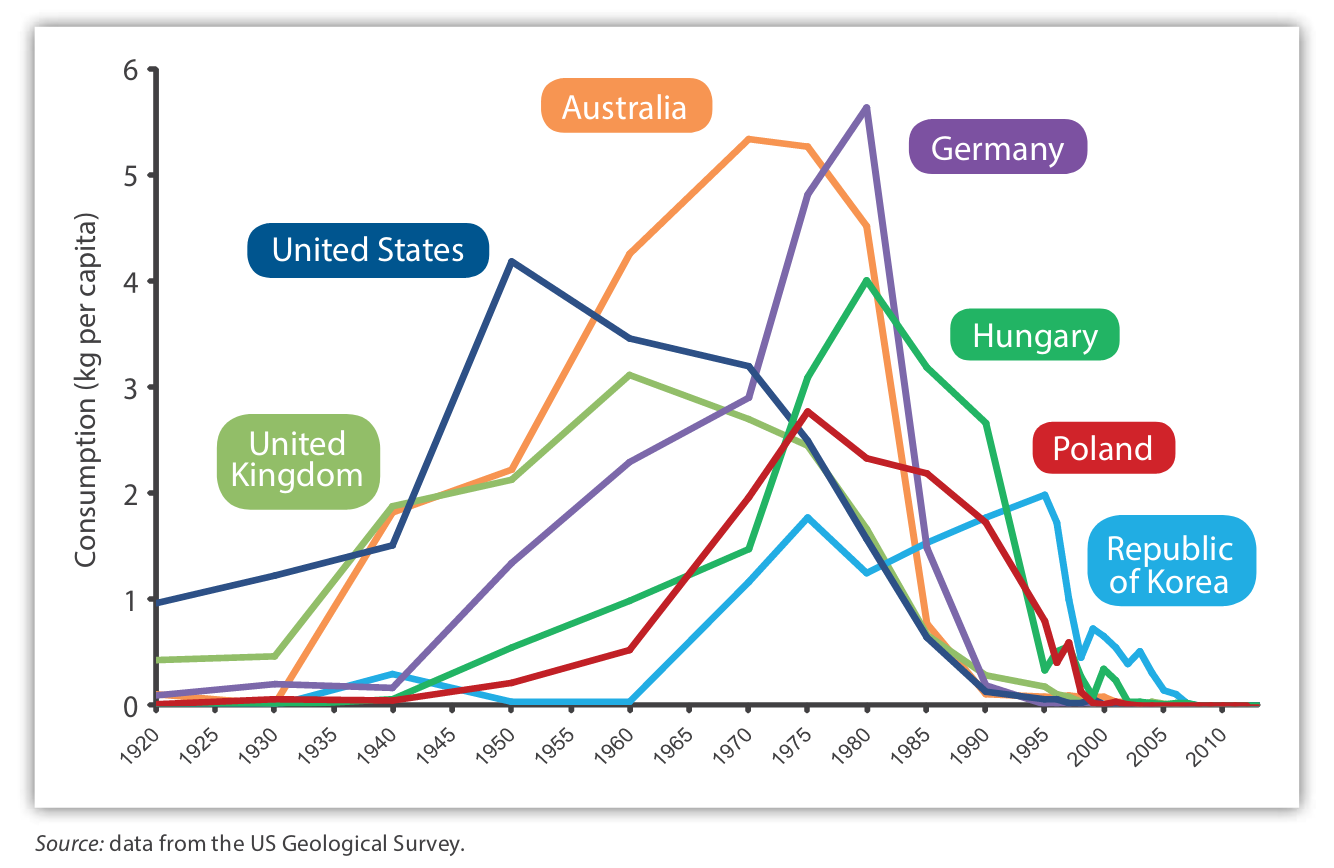
\includegraphics[width=0.5\textwidth,height=\textheight]{source/figures/asbestos_consumption.png}
\caption{Global asbestos consumption per capita 1920-2013}
\end{figure}

The main strengths of our study include its size, use of hospital
controls, high participation rates and avoidance of non-response bias,
the use of two independent validated asbestos exposure assessment
instruments, and the assessment of gene-environment interaction.
Additionally assessors in IPFJES were blind to case status throughout
and the study design and pre-specified outcomes were recorded on
clincialtrial.gov (NCT03211507).

\hypertarget{conclusion-4}{%
\subsection{Conclusion}\label{conclusion-4}}

The majority of men in their 70s in the UK who attend hospital have held
a high or medium risk for asbestos exposure job during their working
lifetime; estimated asbestos exposure based on validated means inferred
by job title or historic asbestos exposure reconstruction methods does
not significantly affect risk of IPF. Nonetheless, about 8\% of IPF
cases have a history of heavy occupational asbestos exposure
(\textgreater25 fibre-ml.years) that would support a diagnosis of
asbestosis based on the Helsinki criteria.

Asbestos exposure alone does not appear to be an important cause of IPF.
It remains possible that it is important in concert with other,
unmeasured, environmental or genetic risk factors, and is associated
with dyspnoea in our study.

\hypertarget{conclusion-5}{%
\section{Conclusion}\label{conclusion-5}}

\hypertarget{thesis-summary}{%
\subsection{Thesis summary}\label{thesis-summary}}

This thesis presents the findings of an analysis of UK mortality trends
for IPF and asbestos related disease, a review of previous occupational
case-control studies of IPF that have investigated occupational
exposures in IPF, a review of historic asbestos exposure assessment
methods, a review of the IPF genetic susceptibility factor MUC5b
promotor region SNP rs35705950, and the idiopathic pulmonary fibrosis
job exposures study (IPFJES).

IPF mortality and asbestos related disease are strongly, if
ecologically, correlated and there are several prima facae reasons to
suppose that occupational asbestos exposure is an under-recognised cause
of IPF, namely: it is more common in men and manual workers, it has been
associated with occupational metal, wood, and stone dust exposures in
several previous studies, and heavy asbestos fibre burdens have been
identified in the lung tissue of IPF patients in a small case series.

Historic asbestos exposure assessment is challenging because of a
paucity of historic data and variable biopersistence and invitro
modification of asbestos fibres. Among the best current validated means
are assessment based on job title and the use of known job title related
pleural mesothelioma risk as a proxy, and historic exposure
reconstruction using source receptor models that provide validated
estimates of cumulative asbestos exposure.

The MUC5b promotor region SNP rs357950 is the strongest identified risk
factor for IPF. It is associated with higher levels of distal airway
MUC5b and is thought to mediate disease by reduced airway clearance and
through interaction with airway microbiota.

IPFJES, a large multicentre hospital based case-control study of
occupational exposures in IPF, demonstrates that the majority of men in
the UK have at least one high or medium risk for asbestos exposure job
during their lifetime and about 8\% have heavy (\textgreater25
fibre-ml.year) asbestos exposure, that this is not significantly
associated with IPF risk, and that this association is not modified by
rs357950 genotype. IPFJES finds a significant association between
occupational asbestos exposure and dyspnoea which is independent of case
and smoking status.

\hypertarget{future-work}{%
\subsection{Future work}\label{future-work}}

Planned future work includes further study of non-asbestos occupational
exposures in IPF, augmentation of the study data with pulmonary function
test measurements, a mendelian randomisation study of smoking in IPF,
and antibody characterisation of serum collected from participants with
a view to investigating the possibility of chronic hypersensitivity
pneumonitis IPF misclassification.

\hypertarget{appendix-1-ipf-epidemiology-code}{%
\section*{Appendix 1: IPF epidemiology
code}\label{appendix-1-ipf-epidemiology-code}}
\addcontentsline{toc}{section}{Appendix 1: IPF epidemiology code}

\href{https://github.com/drcjar/pypf}{IPF epidemiology}

\hypertarget{appendix-2-ipfjes-study-documentation}{%
\section*{Appendix 2: IPFJES study
documentation}\label{appendix-2-ipfjes-study-documentation}}
\addcontentsline{toc}{section}{Appendix 2: IPFJES study documentation}

\href{https://github.com/drcjar/ipfjes/}{IPFJES study documentation}

\footnotesize

\hypertarget{references}{%
\section{References}\label{references}}

\end{document}
